%CLASSE DOCUMENTO - LINGUA E DIMENSIONE FONT
\documentclass[corpo=11pt,numerazioneromana]{toptesi}

%%%%%%%%%%%%%%%%%%%%%%%%%%%%%%%%%%%%%%%%%%%%%%%%%%%%%%%%%%%%%%%

% INCLUSIONE PACCHETTI
\usepackage[classica]{topfront}
\usepackage[utf8]{inputenc} %utf8
\usepackage[italian]{babel}
\usepackage[T1]{fontenc}
\usepackage{blindtext}
\usepackage{graphicx,wrapfig}
\usepackage{booktabs}
\usepackage{lmodern}
\usepackage{varioref}
\usepackage{url}
\usepackage{array}
\usepackage{paralist}{\obeyspaces\global\let =\space}
\usepackage{verbatim}
\usepackage{subfig}
\usepackage{tabularx}
\usepackage{amsmath}
\usepackage{amsfonts}
\usepackage{float}
\usepackage{amssymb}
\usepackage{multicol}
\usepackage{multirow}
\usepackage{listings}
\usepackage[pass]{geometry}
\usepackage[figuresright]{rotating}
\usepackage{algorithm}
\usepackage{algorithmic}
\usepackage{amsmath}
\usepackage[babel]{csquotes}
\usepackage{hyperref}
\usepackage{fancyhdr}

%% this for both bibliography and sitografia
% \usepackage[round]{natbib}
% \usepackage{multibib}
% \newcites{Math}{Sitografia}

%% only bibliography
%%%%5 style=numeric-comp
\usepackage[backend=biber, bibencoding=utf8, style=numeric-comp]{biblatex}
% \usepackage[backend=biber, bibencoding=ascii]{biblatex}

%%%%%%%%%%%%%%%%%%%%%%%%%%%%%%%%%%%%%%%%%%%%%%%%%%%%%%%%%%%%%%%

%INTERLINEA
\interlinea{1.5}

%%%%%%%%%%%%%%%%%%%%%%%%%%%%%%%%%%%%%%%%%%%%%%%%%%%%%%%%%%%%%%%

% CONFIGURAZIONE LINK E RIFERIMENTI
\hypersetup{%
    pdfpagemode={UseOutlines},
    bookmarksopen,
    pdfstartview={FitH},
    colorlinks,
    linkcolor={black}, %COLORE DEI RIFERIMENTI AL TESTO
    citecolor={blue}, %COLORE DEI RIFERIMENTI ALLE CITAZIONI
    urlcolor={blue} %COLORI DEGLI URL
}

%%%%%%%%%%%%%%%%%%%%%%%%%%%%%%%%%%%%%%%%%%%%%%%%%%%%%%%%%%%%%%%

% CONFIGURAZIONE LISTATI/CODICE - CANCELLARE SE NON NECESSARIO
% PYTHON - BIANCO E NERO
\lstset{%
	captionpos=b,
	language=Python,
	basicstyle =\small\ttfamily,
	keywordstyle=\color{black}\bfseries,
	breaklines=true,
	breakatwhitespace=true,
	frame=lines,
	numbers=left,
	numberstyle=\footnotesize,
}

%%%%%%%%%%%%%%%%%%%%%%%%%%%%%%%%%%%%%%%%%%%%%%%%%%%%%%%%%%%%%%%

% FRENCHSPACING VA _SEMPRE_ ABILITATO PER DOCUMENTI IN ITALIANO
\frenchspacing

%%%%%%%%%%%%%%%%%%%%%%%%%%%%%%%%%%%%%%%%%%%%%%%%%%%%%%%%%%%%%%%

%DEFINIZIONE SEZIONI IN NUMERAZIONE ROMANA
%ELENCO DEI LISTATI/CODICI
\makeatletter
\newcommand\listofcodes{%
 \iffrontmatter\else\frontmattertrue\fi
 \if@openright\cleardoublepage\else\clearpage\fi
 % change the meaning of \chapter in a group
 \begingroup\def\chapter##1{\@schapter}
 \phantomsection % for the hyperlink
 \addcontentsline{toc}{chapter}{Elenco dei listati}
 \lstlistoflistings
 \endgroup
} 
\makeatother

\addto\captionsitalian{%
  \renewcommand{\lstlistlistingname}{Elenco dei listati}%
  \renewcommand{\lstlistingname}{Listato}%
}

%%%%%%%%%%%%%%%%%%%%%%%%%%%%%%%%%%%%%%%%%%%%%%%%%%%%%%%%%%%%%%%

%%%%%%%%%%%%%%%%%%%%%%%%%%%%%%%%%%%%%%%%%%%%%%%%%%%%%%%%%%%%%%%

%%% LISTA DEI CAPITOLI DA INCLUDERE - PERSONALIZZARE
\includeonly{%
introduzione,%
chap_1,%
chap_2,%
chap_3,%
conclusioni,%
app_a,%
}

%%%% FILE DI BIBLIOGRAFIA
\addbibresource{bibliography.bib}


%%%%%%%%%%%%%%%%%%%%%%%%%%%%%%%%%%%%%%%%%%%%%%%%%%%%%%%%%%%%%%%



% INIZIO DOCUMENTO
\begin{document}


%%%%%%%%%%%%%%%%%%%%%%%%%%%%%%%%%%%%%%%%%%%%%%%%%%%%%%%%%%%%%%%


%%% REFERENZE
% This is a reference to a chapter \ref{chap:chap_2}. This is a reference to a figure \ref{fig:doge}. This is a reference to some code \ref{lst:hello}. This is a citation \cite{famous:paper}.


\frontmatter

% CITAZIONE - PERSONALIZZARE
% VSPACE - PROPORZIONE USATA PER CENTRATURA VERTICALE DEL TESTO
% FLUSHRIGHT - ALLINEAMENTO ORIZZONTALE A DESTRA
% \vspace*{\stretch{1}}
% \begin{flushright}
% \noindent
% \textit{A Tobia e Bianca}

% \end{flushright}
% \vspace*{\stretch{6}}
% \cleardoublepage



%%%%%%%%%%%%%%%%%%%%%%%%%%%%%%%%%%%%%%%%%%%%%%%%%%%%%%%%%%%%%%%

% ABSTRACT
% \sommario
% Sommario.

%%%%%%%%%%%%%%%%%%%%%%%%%%%%%%%%%%%%%%%%%%%%%%%%%%%%%%%%%%%%%%%

% INDICI - ELIMINARE GLI INDICI NON NECESSARI

% INDICE GENERALE
\tableofcontents

% INDICE DELLE FIGURE
\listoffigures

%INDICE DELLE TABELLE
\listoftables

% INDICE DEI CODICI
% \listofcodes
% \include{strumenti-ottici.py}
%%%%%%%%%%%%%%%%%%%%%%%%%%%%%%%%%%%%%%%%%%%%%%%%%%%%%%%%%%%%%%%

\mainmatter

% INCLUSIONE FILE CAPITOLI - PERSONALIZZARE - TENERE COERENTE CON LISTA IN ALTO

\chapter*{Introduzione}

% \textcolor{red}{METTEREI UNA FRASE CHE INTRODUCA IL TEMA CON UNO SGUARDO PIù AMPIO. QUI UNA PROPOSTA MA PUò AMPLIARE A PIACERE\\
% Prevenire gli scarti di produzione è uno dei principali obiettivi in tutti processi produttivi. 
% }

La prevenzione degli scarti di produzione gioca un ruolo molto importante per il miglioramento del rendimento e delle condizioni finanziarie di qualsiasi azienda. \\
In effetti, l'eliminazione dei difetti ha un effetto diretto sul margine di profitto del prodotto e diminuisce il costo della qualità durante la fabbricazione del prodotto. 
Le aziende si sforzano di ridurre il più possibile il tasso di difetti del prodotto mediante un costante controllo ed ispezione in diversi punti del ciclo di produzione. 
\cite{herdt2010maternal} 


La presente tesi concerne l’analisi del processo relativo alla produzione di innerliner, quale componente che riveste lo pneumatico. \\
Il fine del lavoro è lo studio di come prevenire gli scarti di produzione interni allo stabilimento della Pirelli di Settimo Torinese.
La metodologia utilizzata è stata quella di monitorare costantemente la qualità del prodotto; conseguente a un'accurata comprensione della politica aziendale di gestione dei prodotti non conformi, ossia dei prodotti che non rispettano le specifiche richieste. \\
La prima fase della ricerca si è composta da un'accurata analisi di una serie di campioni relativi alla produzione di innerlinner.
Successivamente, attraverso un identificazione delle cause di variabilità ed il controllo degli indici di processo $CP$ e $CPK$, si è cercato di comprendere come ottenere dei prodotti conformi alle specifiche tecniche stabilite nel piano di controllo. \\
Lo scopo aziendale è quello di assicurare che il processo di produzione e di controllo sia in grado di garantire la conformità del prodotto. 
Ci si riferisce, quindi, sia ai prodotti finiti (lo pneumatico) e sia ai prodotti definiti semilavorati.
A tal proposito sono stati monitorati i processi interni di qualità nella gestione di scarti e scarti di prodotto finito. 
 

L'obiettivo di questa analisi è analizzare come sarebbe possibile migliorare le prestazioni della produzione di innerliner attraverso un costante utilizzo del controllo statistico di processo: utilizzando misure online, estraendo i dati dallo strumento ottico e definendo un appropriato algoritmo di filtraggio e analisi dei dati per la valutazione del prodotto e del processo.

Al fine di rispondere agli obiettivi illistrati, la presente tesi si articola in tre capitoli. \\
Il primo capitolo, ``Review della letteratura'' è un indagine sulle fonti scientifiche relative al miglioramento di un processo produttivo. \\
Il secondo capitolo, ``La metodologia: dai Big Data all'analisi della capacità di un processo'' da una prima definizione ai ``Big Data'' per poi illustrarne i principali aspetti positivi e negativi. Nella seconda parte di questo capitolo viene illustrata la metodologia statistica che si adopererà nell'elaborato: l'analisi di processo, lo studio della variabiltà e gli indici per misurare la variabilità di un processo. \\
Il terzo capitolo concerne l'analisi empirica rivolta allo studio della produzione di innerliner, questo capitolo si articola in tre step principali: introduzione dell'azienda ed illustrazione del ciclo produttivo di uno pneumatico, strumenti utilizzati e linee guida da seguire per la costruzione di un'analisi di processo; validazione dei dati, analisi esplorativa, costruzione ed elaborazione dell'analisi di processo.

Grazie all’analisi del caso di studio, dopo aver seguito i passaggi descritti nel terzo capitolo, si è compreso il comportamento del processo di produzione di innerliner, quindi, sono state identificate alcune fonti di variabiltà che se, monitorate costantemente potrebbero aiutare nell'obiettivo della prevenzione dei difetti. 

% \textcolor{red}{FORSE DIREI QUALCOSA DI SPECIFICO SULLA METODOLOGIA
% E POI RACCONTEREI LA STRUTTURA DELLA TESI
% \\Infine, alcune considerazioni finali concludono l'elaborato. }
\chapter{Review della letteratura}
\label{chap:Review della letteratura}



Lo studio della capacità di processo è un metodo che combina gli strumenti statistici sviluppati a partire dalla curva Gaussiana e delle carte di controllo, adottando una giusta dose di giudizio ingegneristico per interpretare e analizzare i dati che rappresentano un processo. 
\cite{wooluru2014process}


Attraverso la capacità di processo è possibile analizzare gli effetti di variabilità che si hanno sulla media o sulla dispersione di un processo produttivo in un intervallo di tempo definito.  


I risultati dello studio della capacità di processo potrebbero essere utilizzati per nuove applicazioni progettuali, ispezioni, pianificazione e per migliorare le tecniche di valutazione. 
Si definisce quindi, come uno strumento utile a prevenire i difetti durante il ciclo di produzione mediante: la conoscenza sia dei limiti della macchina/processo sia dei fattori che possono essere controllati e non controllati. 
In qualsiasi operazione di produzione c'è un ammontare di variabilità che si manifesta nel prodotto, determinato da diverse condizioni. 

La capacità di processo è la valutazione di quando un processo è in grado di rispettare i requisiti imposti o la sua abilità di produrre prodotti conformi a delle specifiche tecniche.

Invece, il controllo di processo si riferisce alla valutazione della stabilità del processo nel tempo o alla sua capacità di mantenere nel tempo uno stato di buon controllo statistico. 


Per fare un attento controllo statistico di processo é utile monitorare gli indici di capacità di processo come $CP$ e $CPK$. Quest'ultimi, sono utilizzati per valutare la capacità di un processo produttivo di soddisfare le specifiche richieste per una determinata caratteristica di qualità.
\cite{wooluru2014process}

%%%%%%%%%%%%%%%%%%%%%%%%%%%%%%%%%

\section{Il caso di un'azienda industriale}

Sulla base della letteratura esistente, viene riportato
uno studio sulla capacità di processo eseguito da Sudheer D. Kulkarni et al. 
\cite{DUDEKBURLIKOWSKA2005736}

 L'obiettivo fissato dagli studiosi era quello di ridurre al minimo gli scarti causati da difetti di processo e di prodotto e mantenere il processo sotto controllo.
 Questo venne fatto verificando se il processo fosse in grado di soddisfare i requisiti delle specifiche stabilite.

Il caso riporta l'analisi del processo produttivo del portautensili per alesatura (BTH), utilizzato per la lavorazione dei materiali.
Durante la produzione del BTH è stato riscontrato che questo presentava dimensioni che non rientravano nei limiti di controllo stabiliti, dando così origine a prodotti difettosi. 
Tutto ciò ha portato ad una diminuzione della qualità dei BTH prodotti, aprendo così la strada all'insoddisfazione dei clienti.
 Pertanto, era necessario identificare le cause dei difetti per ridurre al minimo il tasso di scarto e migliorare la qualità, aumentando così la produttività dell'azienda.

Per migliorare i processi produttivi e aumentare la qualità dei prodotti, vengono descritte alcune tecniche, come la fresatura ad alta velocità e la metodologia Six Sigma, che permettono di ottimizzare le condizioni di taglio e ridurre il tasso di scarto, aumentando la produttività dell'azienda.

Il processo di taglio é utile a migliorare la progettazione degli utensili, utilizzati in questa fase produttiva in applicazioni avanzate come la fresatura ad alta velocità (HSM). 
Tuttavia, quest'ultima comporta un'elevata temperatura e lo sviluppo di tensioni che portano a tre specifiche conseguenze: un'usura più rapida dell'utensile; una distorsione della finitura superficiale del pezzo e un aumento del costo dell'utensile. 
Si evince quindi, che la modellazione del processo HSM è uno sviluppo essenziale per migliorare la progettazione degli inserti e ottimizzare le condizioni di taglio.

Riprendendo la già citata tecnica Six Sigma si possono definire come delle specifiche metodologie utilizzate per identificare le cause dei problemi di produzione, aumentare la capacità del processo di produrre prodotti conformi alle specifiche richieste e migliorare la soddisfazione dei clienti.

All'interno di questa tecnica, vi è un ciclo di miglioramento definito DMAIC (Definizione, Misurazione, Analisi, Miglioramento, Controllo) composto da cinque fasi:
\begin{itemize}
    \item Definire: identificare il problema da risolvere e definire gli obiettivi del progetto.
    \item Misurare: raccogliere dati sul processo e analizzarli per comprendere le cause dei problemi.
    \item Analizzare: analizzare i dati per identificare le cause radici dei problemi e determinare le soluzioni possibili.
    \item Migliorare: sviluppare e implementare soluzioni per migliorare il processo.
    \item Controllare: monitorare il processo per garantire che le soluzioni siano efficaci e rimanere in linea con gli obiettivi di qualità;
\end{itemize}

L'obiettivo finale di Six Sigma e dell'approccio DMAIC è di migliorare la qualità dei prodotti e dei servizi, ridurre i costi e aumentare la soddisfazione del cliente.
\cite{LeanSixSigma}


Le prime analisi statistiche sono iniziate selezionando le caratteristiche critiche per la qualità. 
Quest'ultime sono state raccolte ed analizzate attraverso vari strumenti di controllo che comprendono: la raccolta; l'analisi dei dati e il miglioramento.
Il corretto utilizzo di questi strumenti prevede una prima costruzione del diagramma a lisca di pesce; per proseguire poi con un'analisi sia dei meccanismi fisici sia della varianza ed infine tramite il calcolo degli indici di capacità del processo, ovvero $CP$, $CPK$, $CPM$.


Questo ha permesso di identificare le opportunità di miglioramento della qualità e della produttività. Inoltre, sono stati studiati gli scarti presenti durante il processo di fusione, utilizzando uno strumento di controllo specifico.
Dall'analisi delle cause di variabilità è stato riscontrato che il difetto più significativo era il soffio causato da macchinari e materiali.

 Le cause di variabilità sono state elaborate utilizzando il diagramma di Ishikawa e attraverso l'analisi dei modi di guasto e l'analisi degli effetti del processo.
 Per migliorare gli indici di capacità di processo del ciclo, sono stati utilizzati grafici elaborati dalla carta di controllo.


Grazie all'utilizzo delle metodologie sopra discusse, il livello di qualità è migliorato spostando la media del processo al valore target e riducendo le variazioni nel processo di produzione di macchine e pezzi di ricambio. L'implementazione della metodologia Six Sigma ha fornito un quadro di come il tasso di scarto sia stato prima monitorato e poi portato al limite di accettabilità nella produzione. 
 L'analisi della capacità del processo è stata eseguita per l'operazione di alesatura e contemporaneamente è stato controllato in maniera frequente l'efficienza del processo stesso. 


 L'obiettivo di ridurre al minimo gli scarti causati da difetti di processo e di prodotto e mantenere quest'ultimo sotto controllo é stato soddisfatto, raggiungendo i requisiti delle specifiche stabilite, migliorando sia la qualità del prodotto che la soddisfazione del cliente. 
 \cite{KULKARNI2022329}


\section{Il caso delle aziende polacche}

In uno studio elaborato da M. Dudek-Burlikowska, intitolato ``Quality estimation of process with usage control charts type X-R and quality capability of process Cp, Cpk'' vengono enunciati gli aspettivi positivi nell'adozione di un metodo per l'analisi del processo produttivo.


L'obiettivo era di prevenire i difetti di produzione, tramite l'implementazione di una metodologia per ridurre i problemi relativi al monitoraggio e al controllo della qualità, che si verificavano nelle aziende polacche.


Si evince, che il monitoraggio dei processi produttivi è un elemento necessario della politica aziendale in termini di qualità e di miglioramento continuo dell'azienda stessa.
È stata discussa la possibilità di utilizzare tecniche statistiche per compiere una stima in materia di qualità, tra queste rientrano: i piani di campionamento, la progettazione sperimentale, l'analisi della capacità del processo e i piani di miglioramento della produzione. 

Le carte di controllo e gli indici di capacità del processo sono strumenti fondamentali che consentono di scegliere quali attività siano più adeguate nel caso in cui si verifichino problemi durante la produzione. 
Tali attività statistiche consentono di analizzare i dati del processo e ottenere informazioni che portano ad un miglioramento dei prodotti finali.
A tal fine, sono state create carte di controllo di tipo X-R e ci si é avvalsi dell'uso degli dell'indici di capacità del processo $CP$ e $CPK$. 
Dall'analisi è stato dimostrato che la loro applicazione permette di prevenire molti difetti anche nelle prime fasi di produzione.

L'indagine è stata ripetuta quattro volte a distanza temporanea di 5 settimane. 
Si nota nella tabella seguente come i due indici di processo $CP$ e $CPK$ presentino una tendenza a crescere col l'avanzare del tempo.


Nella prima settimana, definita ``Seria A'' i valori di $CP$ e $CPK$ erano rispettivamente 0,889.
Tenendo in considerazione che quando si registrano valori minori di 1, il $CP$ indica che il processo non è in grado di soddisfare le specifiche e il $CPK$ indica che una parte del processo cade oltre ai limiti.

\begin{table}[h]
  \centering
  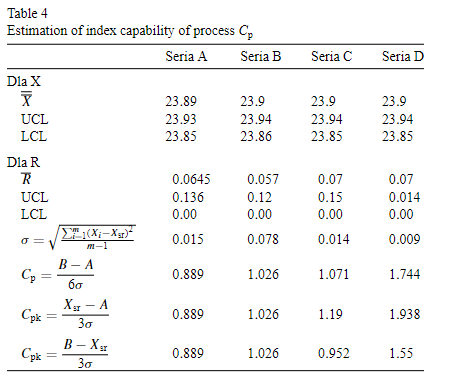
\includegraphics[width=0.85\textwidth]{img/review.png}
  \caption{Indici di capacità di processo} 
  {Fonte: M. Dudek-Burlikowska}
  \label{fig:cp-cpk-review.png}
\end{table}

Con l'avanzare del processo di monitoraggio e controllo di qualità i due indici nell'ultima settimana, ``Seria D'' sono arrivati ad un valore maggiore di 1. 
Questo indica che il processo si è adeguato a soddisfare nel soddisfare le specifiche e che i pezzi prodotti cadono completamente nei limiti di tolleranza. 
\cite{qualityi}


Quindi, l'utilizzo di tecniche statistiche per misurare e migliorare la qualità del processo produttivo, sono d'aiuto nella prevenzione di difetti nel loro successivo rilevamento per migliorare la qualità del prodotto finale.

Si concluse che l'implementazione di tali metodologie statistiche per le aziende polacche sono state efficaci nell'evitare molti difetti di produzione.   
\cite{DUDEKBURLIKOWSKA2005736}



\chapter{La metodologia: dai Big Data all'analisi della capacità di un processo}
\label{chap:Big Data e l'analisi della capacità di un processo}

\section{Big Data}

Con la rapida diffusione della tecnologia dell'informazione, la maggior parte dei dati è diventata quasi totalmente disponibile in digitale. 
Sebbene i progressi dei sistemi informatici e delle tecnologie Internet abbiano visto lo sviluppo dell'hardware di calcolo, i problemi di gestione dei dati su larga scala esistono ancora adesso, nonostante stiamo entrando nell'era dei Big Data.  
\cite{tsai2015big}


I ``Big Data'' sono una grande quantità di dati strutturati e non strutturati che vengono raccolti, archiviati e analizzati per molti scopi, come obiettivi economici e di ricerca.  
\cite{techtarget}


I sistemi che elaborano e memorizzano i Big Data sono diventati una componente comune delle architetture di gestione dei dati nelle organizzazioni, insieme agli strumenti che supportano gli usi analitici dei Big Data. 
Oltre alla questione della dimensione dei dati, Doug  Lancy in una ricerca del 2001 ha presentato una definizione ben nota (chiamata anche 3V) per spiegare cosa sono: volume, velocità e varietà. 
La definizione di 3V implica, rispettivamente, che le dimensioni dei dati sono grandi, che i dati vengono creati rapidamente e che i dati esistono in più tipi e vengono acquisiti da fonti diverse:

\begin{itemize}
    \item il grande volume di dati in molti ambienti
    \item l'ampia varietà di tipi di dati spesso memorizzati nei sistemi di Big Data
    \item la velocità con cui molti dei dati vengono generati, raccolti ed elaborati.
\end{itemize}

Studi successivi hanno sottolineato che la definizione di 3V è insufficiente per spiegare i big data che abbiamo di fronte. Pertanto, per completare la spiegazione dei Big Data sono stati aggiunti veracità, validità, valore, variabilità, vocabolario e vaghezza. 
\cite{tsai2015big}


Con l'aumento delle capacità di archiviazione e la disponibilità di tecnologie avanzate di analisi dei dati, i Big Data stanno diventando sempre più importanti per le industrie manufatturiere.

Uno dei principali vantaggi dell'utilizzo dei Big Data nelle industrie è la possibilità di ottenere una maggiore efficienza nei processi produttivi. Ad esempio, i dati raccolti dalle macchine e dai sensori possono essere utilizzati per ottimizzare i parametri di produzione, ridurre i tempi di fermo macchina e migliorare la qualità del prodotto finale. Inoltre, l'analisi dei dati può aiutare a identificare eventuali problemi nei processi produttivi e a trovare soluzioni efficaci per risolverli.
\cite{Internet4things}


I big data possono anche essere utilizzati per prevedere la domanda del mercato e adattare la produzione di conseguenza, aumentando l'efficienza e riducendo gli sprechi.
Quindi, sono in grado anche di aiutare le industrie manufatturiere a sviluppare nuovi prodotti e servizi. Ad esempio, l'analisi dei dati dei clienti può fornire informazioni sui loro bisogni e preferenze, che possono essere utilizzate per sviluppare nuovi prodotti e servizi. Inoltre, l'analisi dei dati di mercato può aiutare le aziende a identificare nuove opportunità di business. 
\cite{o2015big}

Inoltre, i Big Data possono essere utilizzati per migliorare la sicurezza e la qualità dei prodotti. Ad esempio, l'analisi dei dati di qualità può aiutare a identificare problemi e a prevenire difetti nei prodotti. Inoltre, l'analisi dei dati di sicurezza può aiutare a identificare e prevenire rischi per la sicurezza sul posto di lavoro.
\cite{ThinkOpen}



Tuttavia, è importante notare che per trarre vantaggio dai Big Data, le aziende devono avere una solida strategia e un'adeguata infrastruttura tecnologica. Ciò significa che le aziende devono investire in tecnologie avanzate di raccolta, archiviazione e analisi dei dati, nonché formare il proprio personale per sfruttare al meglio queste tecnologie. Inoltre, le aziende devono essere in grado di gestire e proteggere i dati in modo sicuro, poiché i Big Data possono rappresentare anche un rischio per la sicurezza dei dati.
\cite{BigDataSecurity}



Con l'avvento dei Big Data è nata anche la Data Visualization.
La Data Visualization consiste nella rappresentazione grafica dei dati, in due o tre dimensioni, statica o dinamica. Ci sono molte tecnologie per la Data Visualization che utilizzano elementi visivi come mappe, grafici, barre, ecc. per fornire un modo semplice e intuitivo per visualizzare i dati. Questi strumenti sono utili per identificare situazioni anormali, tendenze o regolarità nei dati. I tool di Data Visualization sono fondamentali nell'industria perché forniscono un'interfaccia user-friendly che è vantaggiosa per la comunicazione tra gruppi operativi con competenze e conoscenze diverse. 
\cite{ScegliFornitore}


In sintesi, i Big Data stanno avendo un impatto significativo sulle industrie manufatturiere. Attraverso l'utilizzo di tecnologie avanzate di analisi dei dati, le aziende possono migliorare la qualità dei prodotti, aumentare l'efficienza e ridurre i costi, sviluppare nuovi prodotti e servizi, migliorare la sicurezza e la qualità dei prodotti, identificare nuove opportunità di business. Tuttavia, è importante notare che per trarre vantaggio dai Big Data, le aziende devono avere una solida strategia e un'adeguata infrastruttura tecnologica. 
\cite{o2015big}

%%%%%%%%%%%%%%%%%%%%%%%%%%%%%%%%%%%%%
\clearpage
\section{L'analisi di processo}
L'analisi di un processo è una metodologia statistica che punta a comprendere e analizzare le variabilità nella qualità di un processo produttivo. 
\cite{qualityi}


L'obiettivo dell'analisi di processo è quello di esaminare la stabilità dei processi attraverso i risultati emersi dagli indici di capacità di processo e valutare la robustezza del processo produttivo per le caratteristiche riportate del piano di controllo di qualità, tramite la definizione di un metodo standardizzato, accompagnato dalla frequenza di campionamento e dalla definizione dei requisiti minimi. 
\cite{blogkainexus}


Per stabilire un metodo standardizzato, è necessario specificare ex ante i metodi di controllo statistico di processo \textit{(Statistical Process Control)}.


Il Controllo Statistico di Processo, detto anche \textit{SPC} può essere descritto come l'utilizzo di una tecnica matematica o statistica che consente di mantenere i risultati di un processo entro specifici limiti, determinati attraverso l'analisi della variabilità intrinseca dei limiti di processo.
Questo sistema di controllo prevede di valutare la capacità del processo all'avvio e periodicamente, e di controllare il suo stato statistico, tramite l'utlizzo sistematico di \textit{Carte di Controllo} per definire, evidenziare e rimuovere eventuali cause che determinano la variabilità.
\cite{WikipediaSPC}


La rilevazione dello scarto quadratico medio, noto anche deviazione standard é uno dei principali metodi statistici applicabili. 
I limiti naturali della variazione di un processo si ricavano attraverso la correlazione tra la deviazione standard e la distribuzione normale.
Un processo viene poi suddiviso in due categorie, in base all'esito del'osservazione:
\begin{itemize}
\item sotto controllo statistico, ovvero quando il processo è influenzato unicamente da fattori casuali, non prevedibili
\item fuori controllo statistico, ovvero quando l'influenza delle variazioni del processo è causata da fattori specifici;
\end{itemize}

In particolare, se si prende in considerazione un processo sotto controllo statistico, effettuando un campionamento di dati, si può notare come il suo andamento temporale seguirà una distribuzione di frequenza che sarà molto simile a una distribuzione normale.


L'analisi del processo dal punto di vista della media e della sua variabilità è fondamentale per determinare i ``limiti naturali" del processo, entro i quali, se non accadono cause specifiche, il processo
manterrà il proprio andamento.
\cite{Joseph}


\begin{figure}[H]
  \centering
  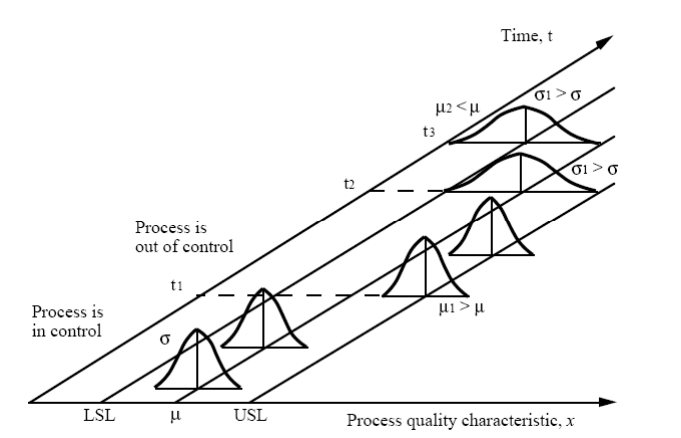
\includegraphics[width=0.75\textwidth]{img/process-quality-char.png}
  \caption{Caratteristiche di un processo statistico} 
  Fonte: Università di Roma, La Sapienza, Dipartimento di Ingegneria Meccanica e Aerospaziale, Programmazione e controllo della produzione, Teoria e metodi del controllo statistico di un processo produttivo
  \label{fig:process-quality-char.png}
\end{figure}

Dall'altra sponda, quando invece, questa distribuzione cambia, oppure variano i limiti, si può pensare ragionevolmente dal punto di vista statistico che stia agendo una ``possibile causa di fuori controllo''.

L'obiettivo, quindi, è quello di ridurre al massimo la variabilità, mantenere il processo sotto controllo, controllare le caratteristiche di qualità durante la produzione. 
\cite{qualityi}
\cite{ManagementAcademy}


%%%%%%%%%%%%%%%%%%%%%%%%%%%%%%%%%%%%%%%%%%%%%%%%%%%%%%%%%%%%%%%%%%%%%%%%%%%%%%%%%%%%%%%%%%%%
\section{Le cause di variabilità}
Per le cause di variabilità é possibile distinguere tra cause comuni o cause cosiddette speciali.
Le cause comuni (o normali), fanno parte del processo e riflettono il processo di variabilità naturale, insorgono casualmente durante il normale svolgimento del processo e ne determinano la fruttuazione naturale.

Tra le cause comuni è possibile identificare la variazione connaturata di materiali grezzi utilizzati nella linea produttiva, la mancanza di adeguata supervisione, i cambiamenti nelle condizioni lavorative e i malfunzionamenti delle macchine.
Bisogna notare che qualsiasi processo comprende delle cause comuni, ovvero un ammontare di ``variabilità naturale''. 

Tra le cause speciali, invece, si trovano le cause che determinano la variabilità non desiderata o anomala rispetto al naturale svolgimento del processo. 
Si tratta di fenomeni anomali che si presentano occasionalmente e possono essere rilevate monitorando continuamente il processo. 
\cite{reconsultsrl}

Le cause speciali possono essere attribuite, ad esempio, da particolari condizioni ambientali, dall'uso di un utensile sbagliato, dall'errore di un operatore o altro. 
Fin quando non verranno rilevate ed eliminate oppure corrette adeguatamente, esse continueranno ad influire in maniera imprevedibile sul processo, portandolo fuori controllo.

A tal fine, un processo sarà definito in base alla presenza o no delle cause speciali. Se in un processo vengono considerate solo la cause comuni di variabilità, eliminando tutte le cause speciali di variabilità: il processo sarà per definizione, ``sotto controllo statistico''.
\cite{qualityi}


\begin{figure}[h]
  \centering
  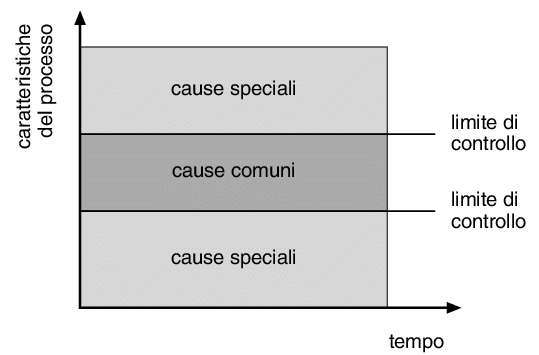
\includegraphics[width=0.75\textwidth]{img/cause.png}
  \caption{Posizione delle Cause di variabilità} 
  {Fonte: \url{https://www.researchgate.net/figure/Cause-comuni-speciali-e-limiti-di-controllo_fig5_289527561}
  Autore: Cristiano Fragassa, Marzo 2007}
  \label{fig:cause.png}
\end{figure}

D'altra parte, se un processo opera considerando anche la presenza della cause speciali, ovvero, fonti di variabilità che non fanno parte delle cause comuni, esso è per definizione, ``fuori controllo statistico''.


Il diagramma di Ishikawa, noto anche come diagramma a lisca di pesce o diagramma causa-effetto, è un ottimo strumento per visualizzare graficamente il potenziale delle cause speciali di uno specifico evento,
Le varia cause sono divise in macro categorie e individuano de percorsi che consentono di raggiungere un obiettivo finale che consiste, appunto, nell'effetto.
I gruppi di cause sono quattro fattori chiave \textit{le 4 M} che influenzano il processo produttivo,
a queste quattro cause fissate da Ishikawa se ne è aggiunta una quinta: l'ambiente, per cui si parla di \textit{5 M}.
\cite{ishi:book}

\begin{itemize}
  \item manodopera
  \item macchine (tecnologia, disponibilità)
  \item materiali (includono i materiali grezzi, consumabili e l'informazione)
  \item metodi (processi)
  \item misure (ispezione, ambiente);
  \end{itemize}


\begin{figure}[h]
  \centering
  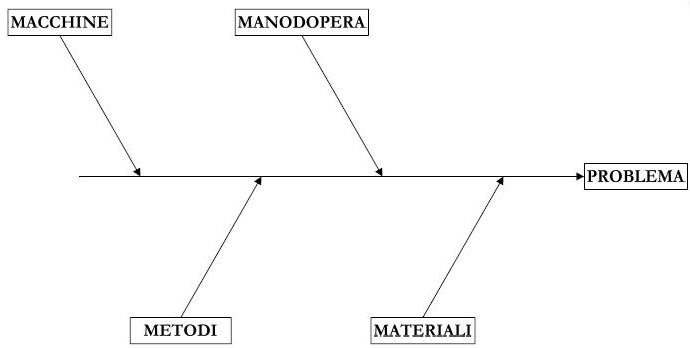
\includegraphics[width=0.75\textwidth]{img/ishikawa.png}
  \caption{Diagramma di Ishikawa} 
  {Fonte: \url{https://it.wikipedia.org/wiki/File:Diagramma_di_Ishikawa.jpg} 
  Autore: Marco Crescenzi, 2008} 
  \label{fig:ishikawa.png}
\end{figure}


In altri termini, si può dire che un processo è fuori controllo quando non segue un andamento casuale e la ragione può essere attribuita ad una delle \textit{5 M} di Ishikawa.

Due delle tecniche statistiche impiegabili nella metodologia SPC sono le carte di controllo e l'analisi della \textit{capability}.
\cite{HumanWare}

%%%%%%%%%%%%%%%%%%%%%%%%%%%%%%%%%%%%%%%%%%%%%%%%%%%%%%%%%%%%%%%%%%%%%%%%%
\section{La carta di controllo}
Molte caratteristiche possono essere espresse sotto forma di misurazione matematica. 

Una singola misura di una caratteristica di qualità, come possono essere, la dimensione, il peso o il volume, viene chiamata variabile.
A tal proposito nasce la Carta di controllo, ovvero, uno strumento utilizzato nell'ambito della statistica per mantenere sotto controllo i vari parametri di un processo. 
\cite{montgomery2009statistical}

La carta di controllo è uno strumento utile anche per monitorare l'evoluzione del processo e capire se un processo e sotto-controllo oppure fuori controllo (presenza o no delle cause speciali).

Se un processo è fuori controllo, la carta di controllo, da un'ipotetica indicazione del motivo del fuori controllo.
Fondamentalmente è una rappresentazione grafica di un processo nel tempo.

Per elaborare una carta di controllo è necessario compiere delle operazioni per un certo numero di campioni, ricavando parametri statistici come media, deviazione standard, range. 

Esistono due macro categorie per le carte di controllo, in base al tipo di dati estrapolati dall'analisi del processo in esame e sui quali sono costruite. 
Vi sono le carte per variabili, utilizzate nel caso di variabili quantitative continue oppure le carte per attribuiti, utilizzate nel caso di variabili quantitative discrete. 
\cite{DiNardo}


Qualora ci si ritrovi a lavorare con una caratteristica di qualità, che è una variabile, sarà necessario monitorare il valore medio della caratteristica e la sua variabilità.
Il controllo del processo in media oppure della qualità della media del processo, tendenzialmente viene fatto tramite la carta di controllo per valori medi. 


Dal lato opposto, la variabilità di processo può essere monitorata o con una carta di controllo per la deviazione standard, detta anche \textit{S control chart} oppure qualora il numero di valori che costituisce la misura è troppo piccolo, affinché la deviazione standard del campione sia statisticamente attendibile viene utilizzata la carta di controllo range, detta anche \textit{R control chart}.
\cite{montgomery2009statistical}


I limiti inferiori e superiori sono calcolati in base ad una distribuzione di frequenza teorica che cambia in funzione del tipo di dati che vengono analizzati, può essere quindi una distribuzione Gaussiana, una Poisson, una binomiale, una T di Student.
Tendenzialmente si utilizza una distribuzione Gaussiana. 
La distribuzione gaussiana, nota anche come distribuzione normale o di Gauss, è una distribuzione di probabilità continuamente utilizzata in molte aree della matematica e della scienza. La sua forma è caratterizzata da una curva a campana simmetrica intorno alla media (o alla mediana), con la maggior parte dei valori concentrati intorno al valore centrale e meno valori estremi. La distribuzione gaussiana è descritta dalla sua media (o mediana) e la sua deviazione standard. La funzione di densità di probabilità per la distribuzione normale è nota come ``funzione gaussiana'' o ``curva normale''.
\cite{WikipediaGauss}



L'attribuzione dei limiti generalmente viene fatta nel modo seguente:

I limiti di controllo sono guidati dalle cause comuni (interne) di variabilità del processo. 
Supponendo che \textit{w} sia un campione statistico che misuri alcune caratteristiche di interesse e supponendo che la media di \textit{w} sia $\mathit{\mu_w}$ e la deviazione standard di \textit{w} sia $\mathit{\sigma_w}$. 

Allora la linea centrale, detta anche \textit{CL: Central Line} che rappresenta la media del processo in controllo, \textit{UCL: Upper Control Limit} che rappresenta il limite superiore di controllo e \textit{LCL: Lower Control Limit}, ovvero il limite inferiore di controllo
si riuniscono nella formazione dei i limiti entro i quali un processo può essere definito in controllo, saranno:


\begin{equation}
  \begin{cases}
  UCL = \mu_w + L\sigma_w\\
  CL = \mu_w\\
  LCL = \mu_w - L\sigma_w \\
\end{cases}
\label {eqn: CONTROL LIMITS}
\end{equation}


Dove \textit{L} è la ``distanza'' riferita ai limiti di controllo, dalla linea centrale \textit{CL}, espressa in termini di scarto quadratico dalla media.
Questo enunciato, è un approccio generale per decidere i limiti di controllo, tuttavia esistono delle specifiche formule che vanno applicate in base alla dimensione del campione e al campo di applicazione.

Una volta definiti i limiti di controllo e osservando la distribuzione del campione di riferimento, sarà possibile individuare eventuali andamenti sistematici dei valori che rappresentano l'evoluzione del processo nel tempo. 

Da qui in poi, saranno poi finalmente visibili andamenti anomali che potranno essere identificabili ad alcune le cause che lo hanno provocato, ad esempio, un andamento ciclico crescente o decrescente della caratteristica misurata, o altri tipi di andamento, trends che rilevano determinate condizioni da correggere, seppur quando le misure restino entro i limiti.

Il processo verrà definito fuori controllo, qualora uno o più punto cadono fuori dai limiti di controllo. 
A tal proposito verranno analizzati i punti che cadono fuori dai limiti di controllo, e verranno adottate delle misure correttive. 
\cite{montgomery2009statistical}


La Carta di Controllo rende possibile comprendere se un processo è fuori controllo (co-presenza di cause speciali) e rilevare eventuali cause speciali di variazione. 
Tuttavia non vengono usate con lo scopo di definire informazioni sulla conformità del processo con limiti di specifica.
L'utilizzo della carta di controllo non è sufficiente a comprendere la reale capacità di un processo nè come questo possa essere migliorato.

In generale, la carta di controllo prende questa forma:
%%% grafico control chart
\begin{figure}[h]
  \centering
  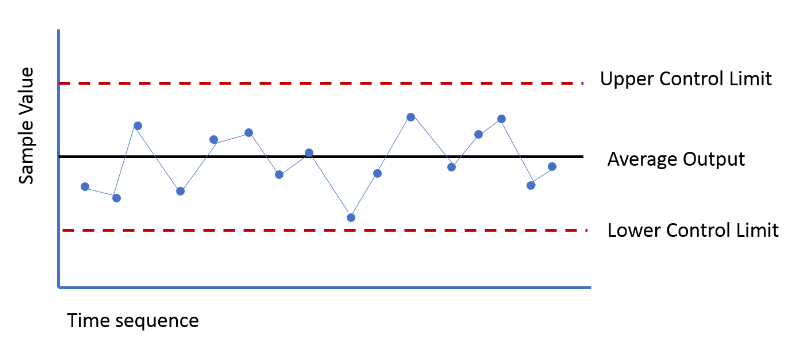
\includegraphics[width=0.85\textwidth]{img/controlchart.png}
  \caption{Carta di controllo con evidenza dei propri UCL/LCL} 
  {Fonte: \url{https://www.zerounoweb.it/analytics/balanced-scorecard-bsc-dinamiche-per-una-data-visualization-mulitimensionale/} Autore: Luigi Buglione}
  \label{fig:controlchart.png}
\end{figure}


Talvolta, possono interessare cose come, le tolleranze di lavorazione o altre specifiche di output del processo. 

La capacità di processo \textit{(process capability)} è una metodologia che, in riferimento ad una determinata attività, operazione, fase o processo caratterizzato da ripetività, consente di valutare quanto un processo produttivo, possa soddisfare una specifica di produzione o specifiche espresse dal cliente in termini di target e di limiti di specifica.
Con lo scopo finale di definire, analizzare e verificare le condizioni che determinano la variabilità dell'oggetto in analisi.
L'essenziale motivo per il quale la capacità di processo è preferibile rispetto ad altre tecniche, viene dal fatto che essa ci permette di valutare, monitorando, due aspetti caratteristici del processo:
\begin{itemize}
  \item la dispersione del processo
  \item la centratura del processo;
  \end{itemize}


Un processo con eccessiva variabilità è distinguibile dal fatto che, un'ampia porzione di area è al di fuori dei limiti di specificazione, nelle due direzioni.
Qualora non vi sia una variabilità elevata, è possibile rilevare un numero di dati esterni ai limiti se il processo non è centrato rispetto al valore di target. 
\cite{UniRoma}




\section{Gli indici di capacità di processo}
Lo studio della capacità di processo è eseguito mediante il calcolo di alcuni indicatori chiave: indice di potenzialità del processo e di prestazione del processo. 
Qualora si abbia a che fare a che fare con un processo stabile (verificato con una quantità di dati indipendenti), la cui variabilità è dovuta solo ed esclusivamente alle cause comuni di variabilità, gli indici utilizzati sono il \textit{Process Capability}, detto anche $CP$ e il \textit{Process Capability Index}, detto anche $CPK$, ovvero indici di potenzialità del processo. 


D'altra parte, qualora i processi con cui si abbia a che fare, abbiano informazioni limitate tali da non poterne ancora definire la stabilità, il $CP$ e il  $CPK$ saranno omessi in funzione di altri due indici, detti $PP$: \textit{Process Perfomance} e il $PPK$: \textit{Process Perfomance Index}, ovvero inidici di prestazione del processo.
In questo caso, non si parla di analisi della capacità di processo ma della capacità di prestazione.
\cite{Meetheskilles}


Con potenzialità del processo ci riferiamo in particolare alla capacità potenziale del processo a mantenere una determinata caratteristica in modo costante all'interno dei limiti di specifica prefissati.

\begin{itemize}
  \item l'indice di potenzialità del processo $CP$, valuta la prestazione quantitativa rapportando l'ampiezza della tolleranza prescritta e l'ampiezza della dispersione del processo.
La variabilità totale è detta anche tolleranza naturale del processo ed è rapportata dal valore $\mathit{6\sigma}$. 

% CP 
L'indice $CP$ è definito come: 
\begin{equation}CP =\frac{UTL-LTL}{6\sigma} 
\label {eqn: CP}
\end{equation}

dove $UTL$ ed $LTL$ sono rispettivamente i limiti di tolleranza superiorori ed inferiori di specifica dati dal piano di controllo e $\mathit{\sigma}$ la deviazione standard del processo calcolata su un numero contenuto di dati (tra 30 e 50).


Il $CP$ è dunque la misura del rapporto tra le dispersione ammissibile per il processo, calcolata dalla differenza tra i limiti di tolleranza, e la dispersione reale, rappresentata da sei volte la deviazione standard, detta anche tolleranza naturale. 
Quindi all'aumentare del valore della deviazione standard, il $CP$ diminuisce.
Questo vuol dire che processi con cause comuni di variazioni molto piccole hanno un elevato valore di $CP$.
\cite{WikCP}



Per una distribuzione normale, l'intervallo compreso tra i due estremi $\mathit{\pm3\sigma}$ include il 99,73\% dei valori di $X$ e, in corrispondenza, si ha il 0,27\% di valori esterni.
Di conseguenza, se l'intervallo di specificazione è maggiore di $\mathit{6\sigma}$ (ovvero se l'indice $CP$ è maggiore di 1) significa, che mediamente si producono meno del 2,7\% di pezzi non conformi e cioè che il processo può ritenersi capace.
Il valore target $CP$ tuttavia, è fissato in base a requisiti specifici di procedure interne, il processo sarà definibile capace qualora il $CP$ è maggiore del target prefissato.
\cite{montgomery2009statistical}

Valori di $CP$ superiori a 1,33 indicano che il processo è adeguato per soddisfare le specifiche. Valori di $CP$  compresi tra 1,33 e 1,00 indicano che il processo processo è adeguato a soddisfare le specifiche ma richiedono uno stretto controllo.
 Valori di $CP$ inferiori a 1,00 indicano che il processo non è in grado di soddisfare le specifiche. Se il processo è centrato all'interno delle specifiche e approssimativamente "normale", allora $CP$ = 1,00 risulta in una frazione non conforme dello 0.27\%. 
 Tale valore è noto anche come potenziale di processo. 
 \cite{Wooluru}
 


L'indice $CP$ è un indicatore efficace della capacità di processo, ma non è sufficiente da solo. 
Il $CP$ controlla solo la dispersione del processo, ma non fornisce informazioni sulla sua centratura. 
Un alto valore di $CP$, che dovrebbe indicare un processo capace, potrebbe in realtà produrre un alto numero di scarti a causa della deriva della media del processo verso i limiti di tolleranza.
Per far fronte a questo problema si introduce l'indice $CPK$.
\cite{qualityi}

\item l'indice di prestazione del processo $CPK$, a differenza del $CP$, considera anche la posizione del processo rispetto ai limiti di tolleranza. Esso considerando anche la centratura del processo, valuta la capacità effettiva di un processo di mantenere una determinata caratteristica in modo costante all'interno dei limiti di specifica prefissati.
Viene calcolato come il minimo tra la distanza del valore medio del processo dal limite di tolleranza superiore rapportato al semintervallo di dispersione e la distanza tra il valore medio dal limite di tolleranza inferiore, rapportato alla stessa quantità. 
\cite{SixSigma}


\begin{equation}CPK = min\left(\frac{UTL-\bar{X}}{3\sigma} ; 
\frac{\bar{X}-LTL}{3\sigma}\right)
\label {eqn: CPK}
\end{equation}

Scegliendo il minore dei due valori a destra e sinistra rispetto al valore medio, è possibile determinare quando il processo è capace sul lato peggiore, ovvero quello rappresentato dalla coda della Gaussiana più vicina al limite di tolleranza. 
\end{itemize}

\begin{itemize}
\item se $CPK$ è negativo, allora quasi la totalità dei pezzi sono fuori tolleranza
\item se $CPK$ è uguale 0, allora la metà dei pezzi prodotti sono fuori tolleranza
\item se $CPK$ è compreso tra -1 e 0, allora più della metà dei pezzi prodotti sono fuori tolleranza
\item se $CPK$ è uguale a 1, si è sul limite della lavorazione di pezzi non buoni
\item se $CPK$ è compreso tra 0 e 1, allora una parte dei pezzi prodotti del processo cadono oltre i limiti
\item se $CPK$ è maggiore di 1, l'ampiezza $\mathit{6\sigma}$ dei pezzi prodotti cade completamente nei limiti di tolleranza, si ha un buon mezzo di lavorazione;
\end{itemize}
\cite{qualityi}


Se l'indice $CP$ risulta uguale all'indice $CPK$ allora il processo è situato esattamente al centro dei limiti delle specifiche.
D'altra parte invece se l'indice $CP$ è diverso dall'indice $CPK$ allora il processo non è sufficiente ed è necessario selezionare un nuovo parametro di processo. 
\cite{yunus2016preliminary}


Gli indici in questione sono preferiti rispetto ad altri metodi statistici e tale motivo è imputabile alla possibilità di riassumere in modo molto coinciso i dati di un processo produttivo, con il vantaggio, di essere facilmente interpretabiili e paragonabili tra loro.
Pertanto, la comodità di tali indici si rende utile per confrontare le capacità di processo relative a differenti tipi di processi. 
\cite{Meetheskilles}

% \begin{figure}[h]
%   \centering
%   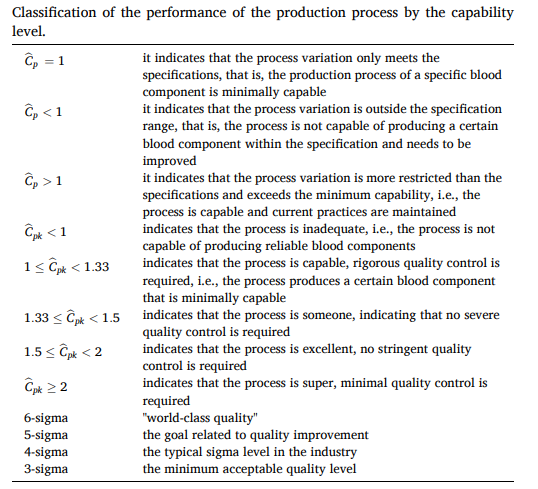
\includegraphics[width=0.85\textwidth]{img/cp-cpk-classification.png}
%   \caption{Classificazione degli indici di capacità di processo} 
%   {Fonte: Process capability indexes: Trends and developments in the manufacturing 
% of blood components, Autore: Paulo Pereira}
%   \label{fig:cp-cpk-classification.png}
% \end{figure}

\chapter{L'analisi empirica}

\section{Storia della Pirelli Industrie Pneumatici}
\label{Storia della Pirelli Industrie Pneumatici}
Pirelli è un'azienda italiana fondata nel 1872 da Giovanni Battista Pirelli. Inizialmente, l'azienda si concentrava sulla produzione di cavi in gomma e fili di rame, ma presto si espandette nella produzione di pneumatici per biciclette e poi per automobili, diventando uno dei principali fornitori di pneumatici in Italia.


Durante la prima guerra mondiale, Pirelli fu un fornitore importante di pneumatici per l'esercito italiano e, nel dopoguerra, si espandette ulteriormente in Europa e in America del Sud. Nel 1923, l'azienda aprì una fabbrica in Argentina e, nel 1926, una fabbrica in Brasile.

Nel corso del XX secolo, Pirelli diventò uno dei principali produttori di pneumatici a livello mondiale, fornendo pneumatici per automobili di lusso, veicoli industriali e veicoli da corsa. Nel 1971, l'azienda venne quotata in borsa e, negli anni successivi, si espandette ulteriormente acquistando altre aziende in Europa e in America del Nord.

Nel 1980, Pirelli acquistò la società americana Armstrong Tire and Rubber Company, che gli permise di entrare nel mercato degli pneumatici per camion e autobus negli Stati Uniti. Nel 1986, l'azienda acquistò la società inglese Armstrong Rubber Company, rafforzando ulteriormente la sua posizione nel mercato europeo.

Negli anni 2000, Pirelli ha continuato a espandersi, acquistando aziende in Asia e in Russia e diventando uno dei principali produttori di pneumatici premium a livello mondiale. Inoltre Pirelli si è distinta nel mondo del motorsport, sponsorizzando e fornendo pneumatici per diverse competizioni di alto livello, tra cui la Formula 1 e la World Rally Championship.

Inoltre, Pirelli ha sempre investito in ricerca e sviluppo, per creare pneumatici sempre più performanti e sicuri. Nel corso degli anni Pirelli ha brevettato diverse soluzioni tecnologiche, come la tecnologia Run-Flat, che permette di continuare a guidare anche in caso di foratura, e la tecnologia EcoImpact, che riduce l'impatto ambientale.

Oggi Pirelli è un'azienda globale con stabilimenti in tutto il mondo e continua ad essere una delle principali aziende nella produzione di pneumatici di qualità per automobili di lusso, veicoli industriali e veicoli da corsa.
\cite{WikipediaPirelli}
\cite{PirelliHist}

%%%%%%%%%%%%%%%%%%%%%%%%%%%%%%%%%%%%%%%%%%%%%%%%%%%%%%%%%%%%%%%%%%%%%%%%%%%%%%%%5
\label{Processo di produzione di uno pneumatico}
\section{Come viene fatto uno pneumatico}

Gli pneumatici sono una caratteristica essenziale per un'ampia gamma di mezzi di trasporto,
la maggior parte dei veicoli, infatti, comprende delle ruote di tipo pneumatico: l'aria è contenuta sotto pressione all'interno dello pneumatico. 
Questi fungonono da superficie di presa per la trazione e da cuscino per le ruote di un veicolo.
Per farla semplice, uno pneumatico è una gomma flessibile attaccata al bordo di una ruota. 

La gomma è il primo materiale essenziale per la costruzione di questo. 
Possono essere anche più di trenta le tipologie di gomme, tra naturale e sintetica, utilizzate per realizzare e definire un nuovo pneumatico.
Oltre alla gomma, vi sono altri materiali come: i plastificanti, il nerofumo e la silice.
Essi sono dedicati e inviati a un mescolatore chiuso, detto \textit{banbury}, all'interno del quale avviene la prima lavorazione della mescola.

La produzione inizia con la miscelazione delle materie prime, come gomma naturale, gomma sintetica e \textit{filler}, per creare un composto di gomma. Questo composto viene quindi estruso attraverso una macchina chiamata \textit{extruder} per formare una striscia di gomma. La striscia di gomma viene quindi arrotolata su un tamburo caldo per darle la forma desiderata.

In una seconda fase di mescolazione, la mescola viene quindi scaricata su un mescolatore aperto composto da due grossi cilindri, al fine di completarne la mescolazione e ottimizzarne la dispersione. 
Dopodichè, la foglia di mescola viene raffreddata in una vasca per il raffreddamento e produrrà quindi un composto più compatto e liscio, detto ``mescola finale''.

Successivamente, la striscia di gomma viene posizionata su una macchina chiamata calandra, dove viene cotto e pressato per dargli la sua forma finale. 
Durante questo processo, vengono aggiunti anche altri componenti come il tessuto di nylon o il filo di acciaio per rinforzare la struttura del pneumatico.
\cite{PirelliComefatto}
\cite{Madehow}

\begin{figure}[H]
  \centering
  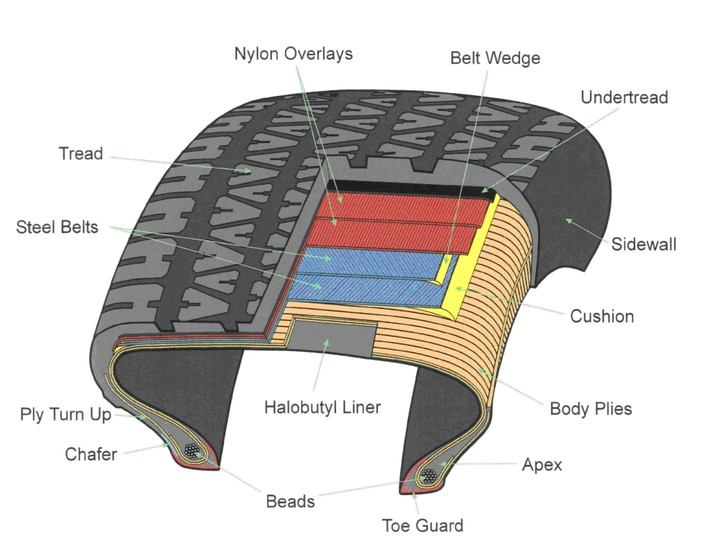
\includegraphics[width=0.65\textwidth]{img/pneumatico.jpg}
  \caption{Componenti di uno pneumatico} 
  Fonte: \url{https://www.pneurama.com/il-rivestimento-interno-dei-pneumatici-che-trattiene-l-aria}
  \label{fig:pneumatico.jpg}
\end{figure}


Il battistrada, ovvero, lo stampo esterno che caratterizza in modo sostanziale lo pneumatico, è un materiale critico nella lavorazione dello pneumatico in quanto il suo ruolo sta nel garantire la frenata su asciutto e bagnato.

Per raffozare lo pneumatico, viene applicato un altro materiale composto da una serie di fili di acciaio, che fornisce rigidità alla zona a contattto con il cerchio: il cerchietto.
Un altro materiale molto importante nella produzione di uno pneumatico sono le tele, che sono essenzialmente dei fili longitudinali e possono essere di vari materali.
Esse vengono quindi tagliate con un certo angolo rispetto alla direzione longitudinale (di marcia, di rotolamento o della trama)

I componenti sinora descritti (battistrada, cerchietti, tele, ecc.) saranno poi portati del reparto di confezione per essere assemblati. 
L'assemblaggio (confezione) dei semilavorati prodotti, viene effettuato secondo precisi criteri qualitativi e specifiche caratteristiche in termini di resistenza e comportamento su strada, è accompagnato quindi da diverse fasi.
Effettuato mediante apparecchiature confezionatrici, l'assemblaggio produrrà quel che si può definire il ``crudo'' dello pneumatico.
Il crudo è poi inviato alla fase successiva di lavorazione: la vulcanizzazione, ovvero una vera e propria reazione chimica condotta in fase solida.

Una volta che lo pneumatico è stato pressato e cotto, viene raffreddato e tagliato per ottenere le dimensioni desiderate. Lo pneumatico viene quindi ispezionato per verificare che soddisfi gli standard di qualità e quindi viene etichettato e confezionato per la spedizione.

La fase del primo controllo concerne in un'ispezione visiva sia interna sia esterna, per verificare eventuali imperfezioni che ne alterino l'aspetto.
Se lo pneumatico non presenta caratteristiche difettose, allora, sarà mandato alle macchine per il controllo di uniformità e bilanciatura, talvolta viene seguito anche da controllo ai raggi X in apposite aree schermate. 
\cite{hilltoptire}
\cite{Madehow}



In conclusione, la produzione di un pneumatico richiede una combinazione di tecnologie avanzate e metodi manuali per garantire che il prodotto finale soddisfi gli standard di qualità e sicurezza. La gomma è l'ingrediente principale per la produzione di pneumatici e deve essere lavorata in modo attento per ottenere un pneumatico resistente e durevole. 

\clearpage
\begin{figure}[h]
  \centering
  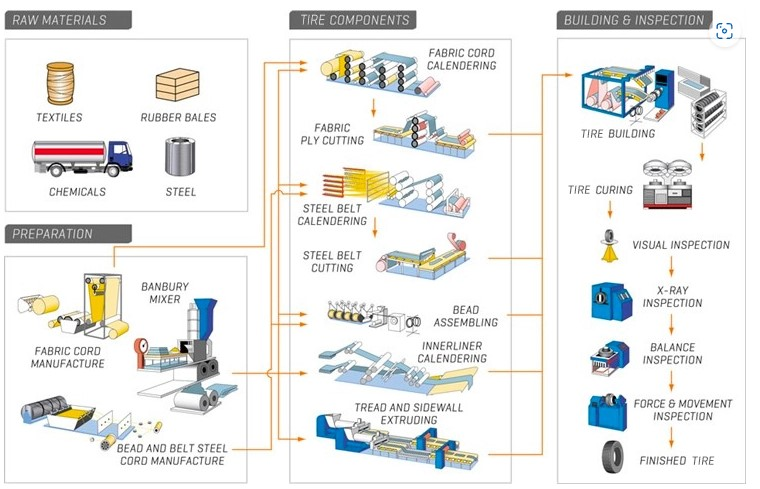
\includegraphics[width=1\textwidth]{img/tyre-process.jpg}
  \caption{Processo di produzione di uno pneumatico} 
  Fonte: \url{https://www.maxxis.com/nl/en/technology/how-a-tire-is-made/} 
  \label{fig:tyre-process.jpg}
\end{figure}



%%%%%%%%%%%%%%%%%%%%%%%%%%%%%%%%%%%%%%%%%%%%%%%%%%%%%%%%%%%%%%%%%%%%%%%%%%%%%%%%%%%%%%%%%%%%%%%%%%%%%%%%%%%%%%
\label{Stumenti utilizzati}
\section{Strumenti utilizzati}


Gli strumenti utilizzati per l'analisi sono stati: Python e JMP.

Python è un linguaggio di programmazione di ``alto livello'', orientato a oggetti, utile a manipolare, filtrare, pulire i dati e fare analisi preliminari (statistiche descrittive), tramite l'utilizzo di alcune librerie. 
Il principale vantaggio associato al linguaggio Python è relativo alla vasta disponibilità di librerie e framework, open-source, che forniscono un supporto efficace in diversi ambiti, dal
machine learning, allo sviluppo di applicazioni web.
La libreria Pandas è ritenuta una delle migliori librerie per l'analisi dei dati. Dispone di potenti strumenti per l'importazione e l'esportazione di set di dati, oltre che per la loro esplorazione, pulizia e analisi. La libreria offre due principali strutture di dati: i DataFrame, che sono strutture bidimensionali con righe e colonne etichettate, e le Serie, che sono array unidimensionali. Queste strutture di dati flessibili e intuitive la rendono una scelta ideale per qualsiasi progetto di analisi dei dati.
\cite{Python}
\cite{PythonPandas}


JMP è un \textit{software} di rilevazione statistica e di Data Visualization lanciato nel 1989 dalla \textit{business unit} JMP dell'istituto SAS;
viene utilizzato in applicazioni quali \textit{Six-Sigma}, controllo di qualità e ingegneria, progettazione di esperimenti, nonché per la ricerca in campo scientifico, ingegneristico e sociale.
JMP è in grado di comunicare con \textit{database} esterni ed è possibile importare dati da un driver ODBC \textit{(Open Database Connectivity)} per il database. 
\cite{WikipediaJMP}


In particolare, nell'analisi del caso di studio, sono stati importati su JMP i dati relativi ad alcuni parametri di processo contenuti nel database dello stabilimento e al fine di condurre una simulazione di risposta, in base a diverse variazioni dei fattori, e cercare di comprendere il problema alla base della capacità di prestazione di una specifica variabile caratteristica della qualità.


\section{Linee guida previste per la costruzione dell'analisi della capacità di processo}
Si è scelto di creare una linea guida per le relative capacità di processo che verranno implementate oppure aggiornate. 
Nel caso preso in esame, i dati analizzati sono misurabili e confrontabili numericamente, quindi si farà riferimento unicamente alle carte di controllo per variabili.
La carta di controllo realizzata, stabilisce tutti i vari requisiti di tolleranza, relativi alle caratteristiche che hanno necessità di essere monitorate.
In questo contesto, sono uscite allo scoperto le prime difficoltà tecniche e i punti di debolezza nel raccoglimento delle informazioni utili.
Per analizzare il punto della situazione, si é proceduto quindi, a classificare il modo in cui vengono tracciati i dati, in tre distinte categorie:
\begin{itemize}
	\item manuale
	\item manuale in laboratorio
	\item automatico;
\end{itemize}

Nella Fig. \ref{fig:capability-level.png} sottostante si é quindi predisposto un grafico a torta sulla base di ció che attualmente si ha all'interno dello stabilimento:

\begin{figure}[h]
  \centering
  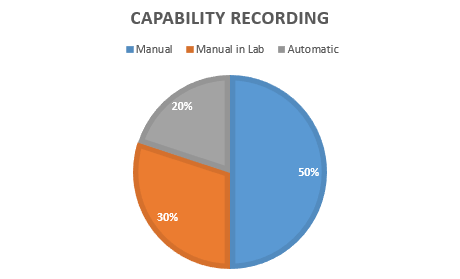
\includegraphics[width=0.75\textwidth]{img/capability-level.png}
  \caption{Tre distinte categorie per il raccoglimento dei dati}
  \label{fig:capability-level.png}
\end{figure}


Dove la fetta colorata in grigio rappresenta il reperimento dei dati in modo automatico e la disponibilità di analisi statistiche elaborate automaticamente. \\
L'inserimento automatico implica una comunicazione perfetta tra macchina e contenitore dei dati, detto \textit{Cloud}, in quanto tutto ció che viene rilevato e scansionato dalle macchine é perfettamente reperibile dagli analisti. \\
In colore arancione é possibile vedere i dati raccolti in modo manuale ed elaborati in laboratorio. \\
La fetta colorata di blu rappresenta i dati raccolti in modo manuale.
Nei casi di raccoglimento dei dati in maniera manuale, la raccolta dati viene effettuata da un operatore di qualità almeno una volta al giorno, l'operatore infatti con il supporto elettronico dato dalla telecamera posta al di sopra della macchina di produzione, procede ad inserire nel database i valori rilevati.

É facilmente visibile che solo una ridotta percentuale delle macchine dello stabilimento fornisce i dati in maniera automatica. 
Questo rappresenta una difficoltà nel raggiungere gli obiettivi di qualità previsti.

Nel piano di controllo sono stati stabiliti anche dei criteri di importanza, ogni parametro rilevato dalle macchine avrà un'importanza diversa rispettivamente ad ogni tipo di semi-lavorato.
Si è quindi proceduto a creare una sorta di gerarchia di importanza di monitoraggio sulle \textit{capability} dei parametri rilevati, per ogni tipo di semi-lavorato.
\begin{itemize}
  \item \textbf{M}: importanza media
	\item \textbf{C}: importanza alta
	\item \textbf{CC}: importanza critica e legale;
\end{itemize}

La classificazione di tipo CC é speciale, in quanto, 
nel caso remoto che un parametro sforasse uno di questi limiti: il prodotto finito non potrebbe uscire dallo stabilimento per essere venduto.
Per agevolare l'analisi, si é predisposto un grafico a torta che rappresenta la situazione nello stabilimento:

\begin{figure}[h]
  \centering
  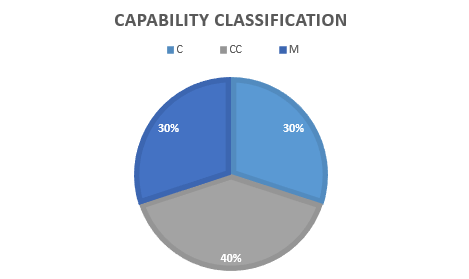
\includegraphics[width=0.65\textwidth]{img/cp-classification.png}
  \caption{Criteri di importanza per i parametri rilevati}
  \label{fig:cp-classification.jpg}
\end{figure}

Le caratteristiche CC e C, verranno dette anche \textit{mandatory} e sono quelle a cui faremo particolare riferimento in quest'analisi, in quanto caratteristiche obbligatorie da monitorare, stabilite dal piano di controllo.

La pianificazione operativa delle attività di controllo della qualità é attualmente un processo chiave non solo per garantire la qualità dei processi realizzati, ma anche per eseguire le attività in condizioni controllate e in regimi di qualità certificata.
In mancanza di un rigoroso controllo qualità, il rischio é quello di immettere sul mercato prodotto difettosi o con prestazioni non adeguate rispetto agli standard stabiliti.
Un piano dettagliato di controllo e garanzia della qualità, permette di ridurre i costi sostenuti dall'azienda (scarti, resi, rilavorazioni) e i rischi di produzione per garantire che tutti i materiali, i processi e i prodotti finiti siano all'altezza degli standard di qualità previsti.
Ad ogni macchina, quindi, corrisponde un relativo spazio nel piano di controllo qualità.

%%%%%%%%%%%%%%%%%%%%%%%%%%%%%%%%%%%%%%%%%%%%%%%%%%%%%%%%%%%%%%%%%%%%%%%%%%%%%%%%%%
\section{Le cause di variabilità riviste per l'analisi}
Sulla base di precedenti analisi fatte da altri stabilimenti, le cause di variabilità (le cause comuni) ovvero le \textit{5 M} di Ishikawa sono state poi riviste implementandone altre tre, rinominando il tutto: \textit{le 8 M}.  
\begin{itemize}
  \item missione/madre natura (scopo, ambiente)
  \item management 
  \item manutenzione (difesa degli obiettivi);
  \end{itemize}


Nell'analisi delle cause speciali, sono sorte alcune delle domande, tali da essere prese in considerazione per indagare in modo specifico sulle cause principali:
\begin{itemize}
  \item Ci sono problemi con l'accuratezza delle misurazioni relative agli strumenti utilizzati?
  \item Ci sono differenze nelle metodologie di misurazione usate da operatori differenti?
  \item I campioni sono stati presi in parti diverse del processo?
  \item Il processo è condizionato da condizioni ambientali? (temperatura, umidità, ecc.)
  \item Nel processo hanno lavorato operatori nuovi, non formati opppure con poca esperienza?
  \item Ci sono stati dei cambi negli \textit{input} di processo? (es. materie prime, ecc.)
  \item Ci sono state delle variazioni nella sorveglianza del processo o nelle procedura?
  \item I parametri di processo sono cambiati?
  \item Ci sono stati cambiamenti significativi nell'ambiente dove il processo veniva effettuato?
  \end{itemize}





%%%%%%%%%%%%%%%%%%%%%%%%%%%%%%%%%%%%%%%%%%%%%%%%%%%%%%%%%%%%%%%%%%%%%%%%%%%%%%%%%%%%%%%%%%%%%%%%%
\label{L'innerliner}
\section{L'innerliner}
L'innerliner è una parte interna di uno pneumatico che si trova tra la carcassa e la camera d'aria. È realizzato in gomma butilica, un tipo di gomma che non si scolorisce o si deteriora facilmente. \\
La funzione dell'innerliner é di mantenere la pressione della camera d'aria all'interno dello pneumatico, ovvero evitare che l'aria fuoriesca dallo pneumatico. 
\cite{Innerliner} \\
Inoltre, l'innerliner aiuta a proteggere la carcassa dello pneumatico dall'ossidazione e dalla corrosione dovute all'umidità e all'ossigeno presenti nell'aria. 
L'innerliner é un componente fondamentale in quanto fornisce una maggiore sicurezza e stabilità allo pneumatico durante la guida. 
\cite{pneurama}
La sua produzione avviene utilizzando una macchina chiamata ``calandra''. \\
La calandra è una macchina industriale che utilizza rulli caldi per miscelare e stendere la gomma butilica per creare una striscia di gomma sottile e continuativa. 
La striscia di gomma viene poi arrotolata e immagazzinata in bobine, che vengono utilizzate per creare l'innerliner dello pneumatico. Il processo di creazione dell'innerliner è molto preciso e richiede una costante attenzione per ottenere una qualità e una uniformità adeguati.
\cite{pneurama}

%%%%%%%%%%%%%%%%%%%%%%%%%%%%%%%%%%%%%%%%%%%%%%%%%%%%%%%%%%%%%%%%%%%%%%%%%%%%%%%%%%%%%%%%%%%%%%%%%%%%%%%%%%%%%%%%
\label{Gli strumenti di rilevazione dei parametri}
\section{Gli strumenti di rilevazione dei parametri}
L'analisi e lo sviluppo del caso di studio sulla capacità prestazionale sono stati possibili grazie alle misure eseguite dagli strumenti ottici posti al di sopra della calandra.
Quest'ultimi forniscono un importante contributo per una maggiore efficienza e qualità nel processo di controllo della produzione di pneumatici.
Alcuni parametri dell'innerliner che vengono monitorati durante la produzione sono:

\begin{enumerate}
\item sistemi di controllo della temperatura
\item sistemi di misura dello spessore
\item sistemi di misura della larghezza
\item sistemi di rilevamento delle bolle d'aria: per individuare eventuali bolle d'aria nell'innerliner durante la produzione, in modo da poterle rimuovere prima che lo pneumatico venga montato.
\item sistemi di rilevamento della velocità della linea
\item sistemi di registrazione dati: per tracciare e registrare i parametri dell'innerliner in modo da poterli utilizzare per eventuali analisi future o per ottimizzare il processo di produzione;
\end{enumerate}

Tutti questi sistemi lavorano in sinergia per garantire che l'innerliner sia di qualità e soddisfi i requisiti di sicurezza e di prestazioni richiesti dal produttore.

Nella Fig. \ref{fig:profilometro.jpg} é possibile vedere con precisione il modo in cui lo strumento ottico rileva tali parametri.
Lo strumento é in grado di misurare con precisione, tramite cinque differenti punti la larghezza dell'innerliner e il relativo spessore di ognuno dei due strati.


\begin{figure}[h]
  \centering
  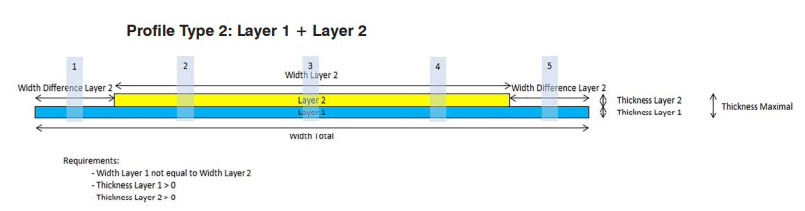
\includegraphics[width=1\textwidth]{img/profilometro.png}
  \caption{Misurazioni dallo strumento ottico}
  \label{fig:profilometro.jpg}
\end{figure}


I dati estratti dallo strumento ottico, vengono raccolti in formato csv e salvati in cartelle.
Vi é una particolare differenza nel modo in cui vengono raccolti ed archiviati i dati, si avranno quindi i dati registrati in locale dalla macchina e i dati trasmessi dai dispositivi integrati IIoT, quest'ultimi verranno semplicemente definiti come dati IIoT.
Le reti IIoT tipicamente supportano la comunicazione e la trasmissione regolare di dati tra il sistema centrale e tutti i dispositivi integrati IIoT.
\cite{SAP}



I dati rilevati con la tecnologia IIoT mostrano tutti i parametri rilevati con una frequenza di campionamento non pre-fissata; la tecnologia IIoT permette di registrare i dati solamente qualora vi sia una variazione di almeno uno dei parametri, quindi qualora si fossero mantenuti dei valori costanti in tale arco di tempo, sul csv non saranno riportati tali valori ma attenderanno la variazione di almeno un parametro.

Differentemente si comporta lo strumento che registra i dati in locale, quest'ultimo infatti é soggetto ad una frequenza fissa di campionamento, quindi rileva tali parametri con una frequenza pari a 5 secondi.
Quest'ultimo, a differenza del dispositivo IIoT registra tutti i valori rilevati, anche qualora questi siano stati mantenuti costanti.

Un'altra particolare differenza si nota tra la sincronizzazione in tempo reale dei dati, lo strumento che registra i dati in locale, presenta il difetto di non essere sincronizzato in tempo reale. 
Questo é stato uno dei motivi fondamentali nella scelta dello strumento da utilizzare nell'analisi e nel futuro sviluppo di uno strumento di analisi della capacità di processo che fosse accessibile a tutti in tempo reale.

É importante notare che ad ogni differente pneumatico corrisponderà un diverso codice ricetta di produzione dell'innerliner. 
A tal proposito di fronte ai dati a disposizione sarà necessario chiarire, il tempo che intercorre tra la dichiarazione sul computer disposto fronte macchina di un cambio ricetta e l'effettivo cambio ricetta sulla macchina, al fine di evitare di eseguire l'analisi comprendendo i valori anomali di transizione; in quanto ad ogni differente ricetta corrispondono parametri non identici alla precedente.

Le variabili misurate dallo strumento ottico ammontano a 128, tra le quali è possibile trovare:
\begin{itemize}
  \item larghezza del primo layer in mm
  \item larghezza del secondo layer in mm
   \item totale larghezza misurata
  \item spessore del primo layer in mm
  \item spessore del secondo layer in mm
 \item totale spessore in mm;
\end{itemize}

La larghezza totale e lo spessore dell'innerliner saranno il focus fondamentale di quest'analisi.

L'obiettivo dell'analisi, quindi, è quello di ridurre al massimo la variabilità, mantenere il processo sotto controllo, controllare le caratteristiche di qualità durante la produzione \textit{(on-line)} e correggere le possibili anomalie.


%%%%%%%%%%%%%%%%%%%%%%%%%%%%%%%%%%%%%%%%%%%%%%%%%%%%%%%%%%%%%%%%%%%%%%%%%%%%%%%%%%%%%%%%%%%%%%%%%%%%%%%%%%%%%%
\label{Validazione dei dati}
\section{Validazione dei dati}
La fase di preparazione dei dati, anche nota come pre-elaborazione, è un processo importante che coinvolge la pulizia e la trasformazione dei dati grezzi che verranno utilizzati successivamente per l'elaborazione e l'analisi. Questa fase è cruciale per garantire che i dati siano privi di errori e per selezionare solo quelli di alta qualità che garantiranno prestazioni ottimali durante il processo di elaborazione e analisi.

La preparazione dei dati consiste nella rimozione di distorsioni come dati ridondanti, incompleti o non corretti e nella trasformazione dei dati in informazioni rilevanti. Il processo include anche la standardizzazione dei formati, l'arricchimento dei dati e la rimozione dei valori anomali. In sintesi, la preparazione dei dati è un passaggio fondamentale per garantire l'accuratezza e la qualità delle informazioni utilizzate in seguito nell'elaborazione e analisi. 
\cite{Talend}


 Nell'analisi in questione il processo di preparazione dei dati è risultato essenziale, in quanto ha permesso la trasformazione dei dati grezzi in dati di qualità migliore. 
Per la validazione dei dati forniti da entrambi gli strumenti di raccolta dati, si é deciso di monitorare uno dei due parametri obbligatori o \textit{mandatory} stabiliti dal piano di controllo: lo spessore dell'innerliner.

Non era possibile decidere preventivamente quale dei due strumenti di raccolta dati utilizzare, per cui si è scelto di confrontare, sulla base di un campione, le due diverse distribuzioni dei dati relativi ad una variabile.
La scelta di uno strumento di raccolta dati rispetto ad un altro, infatti verterà anche sulla similarità delle due distribuzioni. Qualora i due strumenti presentino distribuzioni simili, dettate da un valore medio e una deviazione standard molto vicine, allora si sceglierà lo strumento ottico migliore in termini di acquisizione dati.

I dati da analizzare sono dati sequenziali, riferiti ad un intervallo di tempo prestabilito.
L'estrazione dei dati è stata possibile grazie all'utilizzo del linguaggio di programmazione Python, di fronte a quest'ultimo infatti si è reso possibile il collegamento con le due diverse fonti.
Sono state rilevate altre variabili (in totale 128), per cui è stato necessario filtrare sulla base di tutte le colonne che contenevano la variabile dello spessore, \textit{thickness}.

Le variabili sulle quali sono state confrontate le due distribuzioni sono lo spessore del primo layer destro in mm (Thickness Layer 1 (mm) right side) e lo spessore del secondo layer in mm destro (Thickness Layer 2 (mm) right side).

Nel dataset vi erano più tipologie di ricette di produzione dell'innerliner, per cui è stato necessario un filtro per una codice ricetta predefinita. 
La ricetta è stata scelta sulla base dei rilevamenti in tale orario di campionamento, quest'ultima verrà rinominata come ``RIC-37''.
Tutte le operazioni indicate sopra sono state adottate sia per i dati raccolti in locale e sia per i dati IIoT.


Nelle Tab. \ref{fig:table-str1-ric37.png}  e \ref{fig:table-str2-ric37.png} é possibile osservare un campione delle osservazioni rilevate.
Esportando i dati su Excel si è reso possibile notare come il campione cambiava rispetto in base allo strumento di raccolta dati utilizzato: i dati IIoT, infatti registravano 714 campionamenti (N ammontava a 714) mentre per i dati registrati in locale il numero di campionamenti è pari a 456.
Questo è particolarmente giustificato dalla diversa frequenza con il quale i campionamenti vengono registrati, visibile dalla colonna ``t sampling'':

\begin{table}[h]
  \centering
  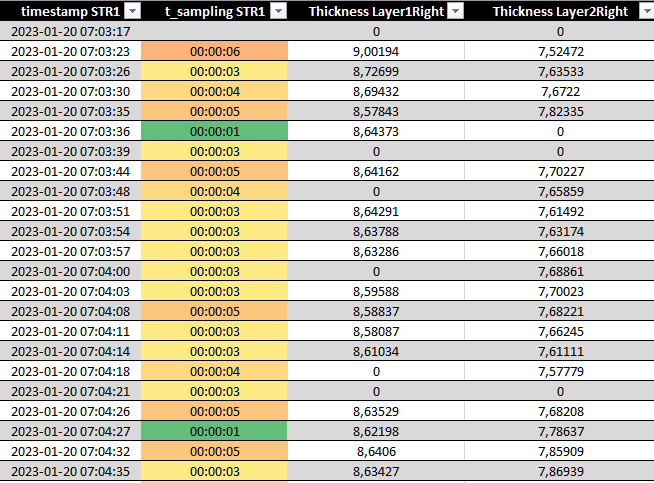
\includegraphics[width=0.7\textwidth]{img/table-str1-ric37.png}
  \caption{Dati IIoT rilevati per la variabile dello spessore}
  \label{fig:table-str1-ric37.png}
\end{table}

Come detto in precedenza, i dati in locale, salvo errori di sincronizzazione, campionano tutte le informazioni con frequenza costante, mentre i dati IIoT registrano i campioni solo a seguito di una variazione.
Per cui può essere ragionevole considerare un fattore di errore per le successive analisi.

\begin{table}[h]
  \centering
  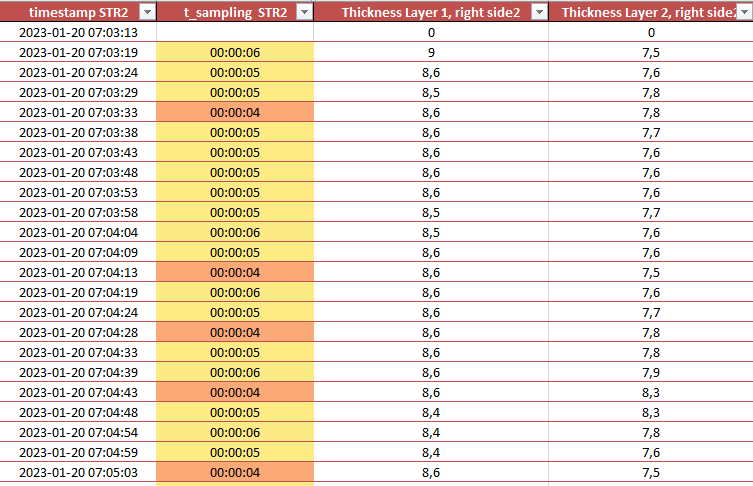
\includegraphics[width=0.7\textwidth]{img/table-str2-ric37.png}
  \caption{Dati in locale rilevati per la variabile dello spessore}
  \label{fig:table-str2-ric37.png}
\end{table}

I due dataset in questione sono stati poi esportati direttamente sul software JMP per ricavare delle analisi descrittive più approfondite.

Per fare delle analisi accurate è stato necessario escludere i valori pari a zero, in quanto generano valori anomali. Questo è stato reso possibile perchè nel caso in questione, un valore pari a zero può indicare o un fermo macchina oppure un problema all'interno dello strumento ottico, che nel caso in questione non ci interessa considerare.


Trasferendo i dati su JMP, quest'ultimo genera la distribuzione di frequenza, un ``boxplot'' e le statistiche descrittive.
Un boxplot è un tipo di grafico utilizzato per rappresentare i dati quantitativi in un formato conciso. Consiste di una ``scatola'' che rappresenta la parte centrale dei dati (cioè l'intervallo interquartile) e due ``code'' che rappresentano i valori più estremi (cioè gli outlier). 
La lunghezza della scatola indica la variabilità dei dati e la posizione della mediana è indicata da una linea orizzontale all'interno della scatola. 
\cite{JMPBoxplot}



Nella Fig. \ref{fig:stat-descr-ric37.png} si notano graficamente dei valori anomali \textit{outlier}, forse relativi al cambio ricetta, ovvero sono stati rilevati i valori transitori relativi alla ricetta precedente.
In futuro, questi valori relativi al cambio ricetta dovranno essere esclusi per l'analisi della capacità di processo e dall'esclusione si vedrà variazione nella media e nella deviazione standard.

\clearpage
\begin{figure}[h]
  \centering
  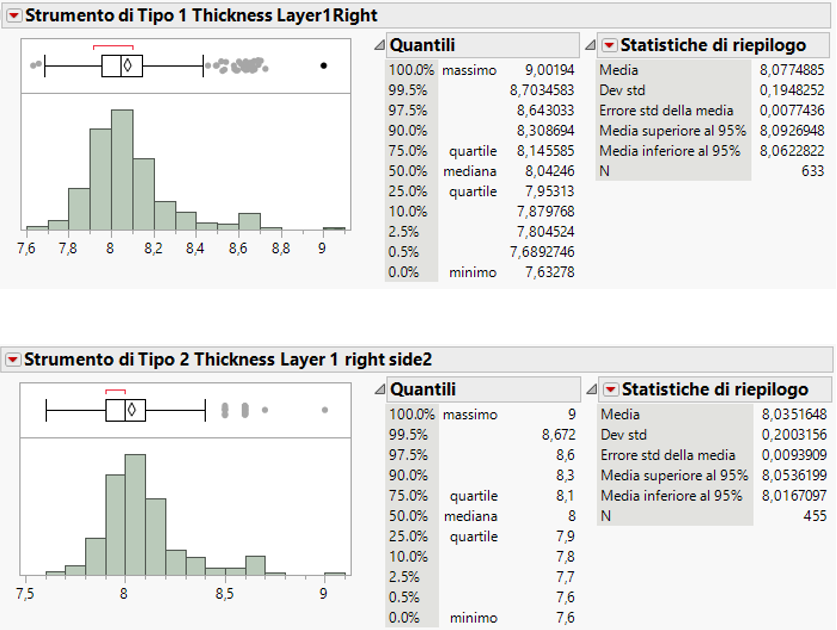
\includegraphics[width=0.8\textwidth]{img/stat-descr-ric37.png}
  \caption{Distribuzione e statistiche descrittive rilevate dai due strumenti ottici}
  \label{fig:stat-descr-ric37.png}
\end{figure}


Al di là della diversa frequenza di campionamento, i due rilevamenti sono simili, la mediana è la medesima e lo scostamento che si ha in termini assoluti contiene medie e varianze simili. 
Pertanto conviene fare lo studio della capacità di processo sui dati IIoT, considerando che vengono campionate più informazioni e i dati sono resi disponibili in tempo reale.


\label{Il campione nell'intervallo di produzione}
\section{Il campione nell'intervallo di produzione}

Per l'analisi si è deciso di estrarre un campione relativo ad una giornata produttiva.
Tale campione durante l'analisi sarà ulteriormente stratificato sulla base della relativa ricetta e su di questo saranno condotte le relative analisi.
Si è scelto preventivamente di monitorare l'andamento di due parametri: la larghezza del secondo strato (layer) sinistro.

\begin{table}[H]
  \centering
  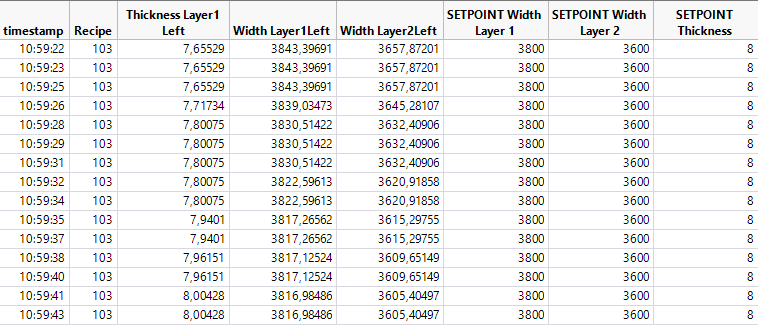
\includegraphics[width=1\textwidth]{img/raw-dati.png}
  \caption{Parte del campione di osservazioni rilevate}
  \label{table:raw-dati.png}
\end{table}

La Tab. \ref{table:raw-dati.png} oltre ai valori misurati di spessore e larghezza, è stata integrata anche dei valori di target stabiliti per codice ricetta, dati da (SETPOINT Thickness / SETPOINT Width) che insieme ai criteri di tolleranza stabiliti, saranno utili per il calcolo degli indici di capacità del processo. \\
Per condurre un'analisi su come si distribuisce ogni campione nel tempo per relativa ricetta, si renderà necessario l'utilizzo di una serie storica. 
Una serie storica è una sequenza di osservazioni ordinate rispetto al tempo. Lo scopo dell’analisi delle serie storiche consiste nello studio dell’evoluzione passata del fenomeno rispetto al tempo. 
\cite{SerieStoriche} \\
L'analisi della serie storica sulla variabile della larghezza è necessaria perchè quest'ultima, rispetto allo spessore, varia al cambiare del codice ricetta dell'innerliner.
Dall'altra parte lo spessore non varia e il target di quest'ultimo sarà sempre 8 mm.  \\
Per non avere problemi di visualizzazione del grafico si è resa necessaria l'esclusione a priori delle osservazioni pari a zero, ovvero i valori nei quali lo strumento è stata fermo.
Per ogni ricetta è stato costruita la relativa serie storica monitorando il parametro della larghezza del secondo layer sinistro, in ascissa vi sarà l'orario corrispondente alla produzione di tale codice ricetta e in ordinata i valori rilevati.   \\
Nelle Fig. \ref{fig:Rec103-Raw-Time.png} e Fig. \ref{fig:Rec105-Raw-Time.png}, verranno mostrate le relative analisi dei primi due codici ricetta per osservare come si distribuiscono nel tempo di produzione campionato.

\begin{figure}[h]
  \centering
  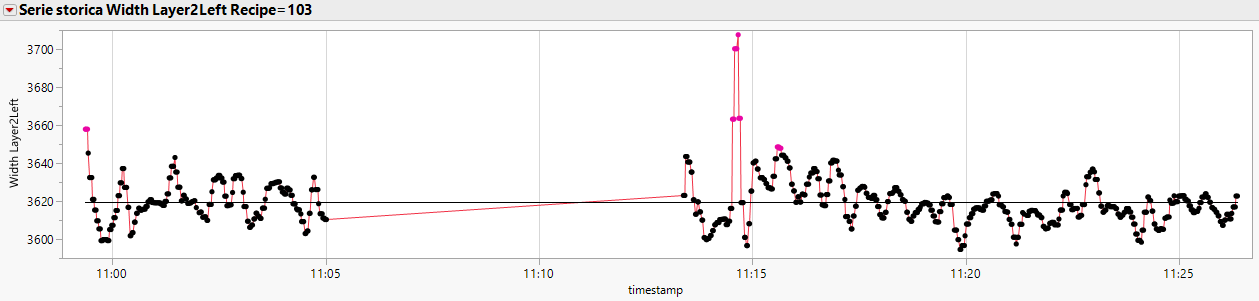
\includegraphics[width=1\textwidth]{img/Rec103-Raw-Time.png}
  \caption{Serie storiche della larghezza per il codice ricetta 103}
  \label{fig:Rec103-Raw-Time.png}
\end{figure}

\begin{figure}[h]
  \centering
  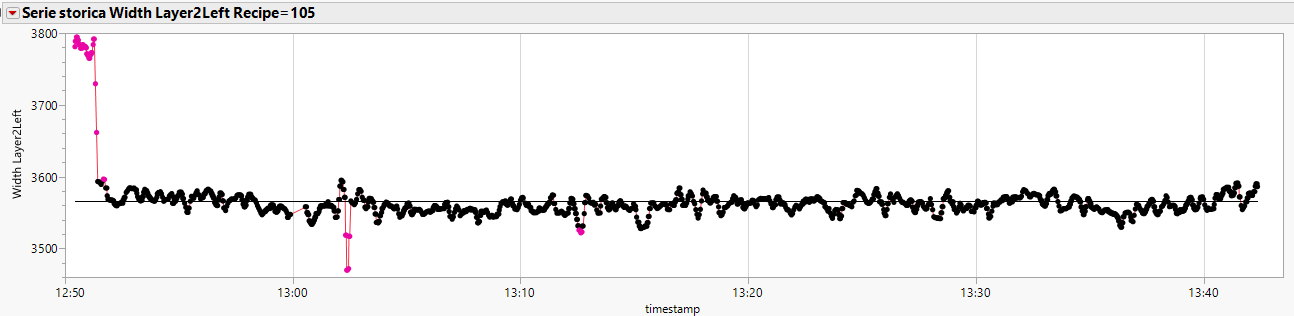
\includegraphics[width=0.90\textwidth]{img/Rec105-Raw-Time.png}
  \caption{Serie storiche della larghezza per il codice ricetta 105}
  \label{fig:Rec105-Raw-Time.png}
\end{figure}

La retta di colore nero in figura mostra la media del processo, mentre i punti indicano le rilevazioni effettuate.
La prima cosa che si nota nelle serie storiche sottostanti è la presenza di valori di transizione anomali ad inizio processo.
I valori di transizione anomali, come spiegato in precedenza sono un insieme di dati che mostra un comportamento insolito all'inizio e alla fine nella produzione di un codice ricetta. 

Questo può essere causato dal ritardo della dichiarazione del cambiamento nella ricetta utilizzata e l'effettivo cambiamento nella macchina, quindi in termini di dati avremo un cambiamento nei valori di misurazione dei parametri considerati. 
Questi cambiamenti possono portare a valori anomali che non riflettono la tendenza generale della serie storica e possono influire sulla capacità di prevedere il futuro.
È importante identificare e gestire questi valori anomali per garantire la validità dei risultati e le conclusioni tratte dai dati.


Per l'identificazione dei valori anomali, ovvero i valori che non riflettono la tendenza generale, si farà uso della distanza interquartile, detta anche IQR.
I valori anomali calcolati con la distanza interquartile sono visibili nelle due serie storiche a partire dai punti di colore rosa.


La distanza interquartile (IQR) è una misura della dispersione dei dati che rappresenta la differenza tra il terzile superiore (Q3) e il terzile inferiore (Q1) di un insieme di dati. Si può utilizzare l'IQR per identificare i valori anomali nel seguente modo: i valori che si trovano al di fuori del range compreso tra Q1 - 1,5 * IQR e Q3 + 1,5 * IQR sono considerati come valori anomali. Questo metodo è adatto per distribuzioni non Gaussiane in quanto non fa alcuna ipotesi sulla forma della distribuzione.
\cite{WikipediaIQR}


A tal proposito, verrà rieseguita l'analisi della serie storica escludendo i valori che non riflettono la tendenza generale unicamente ad inizio e fine rilevazione.
Avendo escluso tali valori anomali sarà più semplice notare in dettaglio il comportamento delle rilevazioni per ogni codice ricetta.


Per il codice ricetta 103, è possibile visualizzare nella Fig. \ref{fig:Rec103-Filtered-Time.png} le rilevazioni del processo.
Si nota facilmente come nella fase centrale del processo, tra le 11:05 e le 11:13 circa, vi sia un interruzione nel rilevamento dei valori, probabilmente causata da un fermo macchina.
Questa è una delle cause speciali di variabilità enunciate nel capitolo \ref{chap:Big Data e l'analisi della capacità di un processo}. 
Durante la produzione, un fermo macchina potrebbe interrompere il flusso del processo, rallentando o bloccando la produzione.
Una volta risolto il problema e ripristinato il funzionamento della macchina, il personale addetto può riprendere il flusso del processo di produzione dell'innerliner. Tuttavia, potrebbe essere necessario un periodo di tempo per raggiungere nuovamente i livelli di produzione precedenti all'interruzione del processo.

Le successive rilevazioni, dopo le 11:13 potrebbero essere ancora in parte influenzate dal ripristino successivo al fermo macchina.
Nella fase successiva del processo, invece sulla curva i punti di osservazione mostrano variazioni significative attorno al suo valore medio. Dunque non è possibile identificare un un comportamento stabile e prevedibile nel tempo.


\begin{figure}[h]
  \centering
  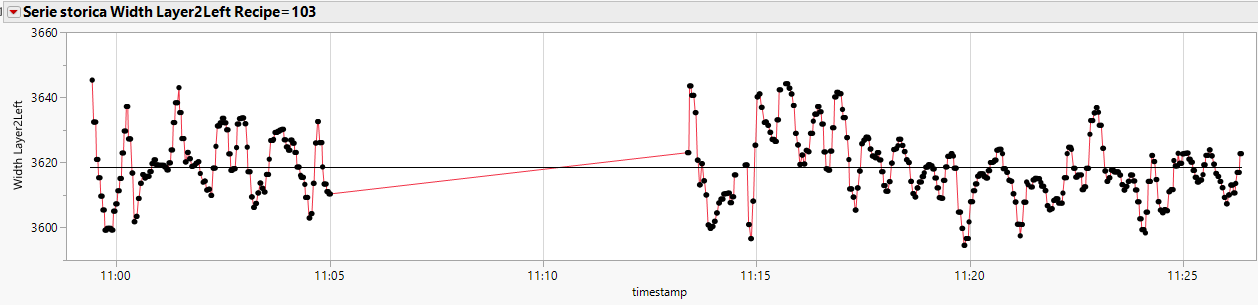
\includegraphics[width=1\textwidth]{img/Rec103-Filtered-Time.png}
  \caption{Serie storica della larghezza per il codice ricetta 103 esclusa dai valori anomali}
  \label{fig:Rec103-Filtered-Time.png}
\end{figure}


La serie storica visibile nella \ref{fig:Rec105-Filtered-Time.png}, relativa al codice ricetta 105, mostra una tendenza centrale ma anche variazioni significative rispetto a questa tendenza. Ciò significa che i valori registrati tendono ad oscillare attorno al valore medio, ma possono anche deviare in modo significativo da questo, sia verso il basso che verso l'alto. 

Tali oscillazioni potrebbero essere dovute a una serie di fattori, come ad esempio la velocità della linea, le condizioni delle attrezzature o altre questioni operative. 
Sarà importante monitorare ulteriormente queste serie storiche per identificare eventuali tendenze o fattori che stanno causando le variazioni e prendere eventuali azioni correttive per migliorare la produzione del codice ricetta.

\begin{figure}[h]
  \centering
  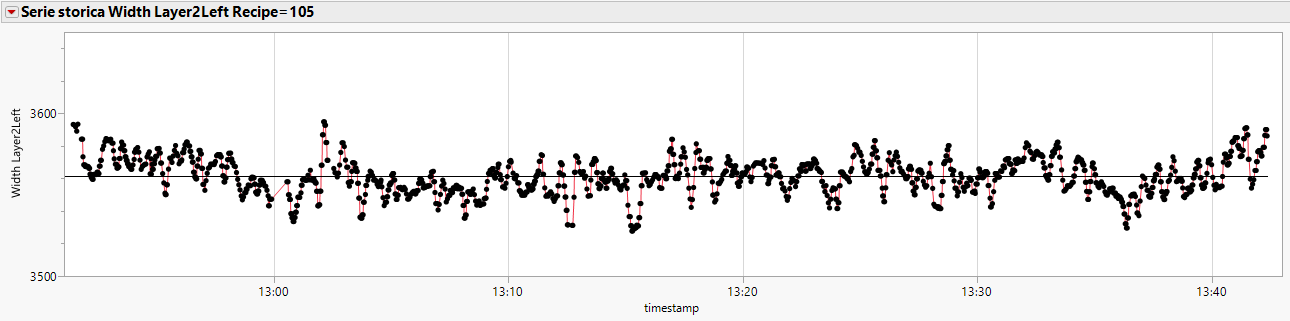
\includegraphics[width=1\textwidth]{img/Rec105-Filtered-Time.png}
  \caption{Serie storica della larghezza per il codice ricetta 105 esclusa dai valori anomalii}
  \label{fig:Rec105-Filtered-Time.png}
\end{figure}


%%%%%%%%%%%%%%%%%%%% 

\label{La distribuzione del campione}
\section{La distribuzione del campione}

Uno dei criteri per condurre l'analisi della capacità di processo è la distribuzione normale dei dati.
In statistica, i test di normalità vengono utilizzati per determinare se un insieme di dati ha la forma di una distribuzione normale e per calcolare quanto sia probabile che una variabile casuale sottostante l'insieme di dati sia normalmente distribuita.
\cite{KULKARNI2022329}


Poichè il criterio è necessario per effettuare l'analisi della capacità di processo, si è predisposto un test di normalità.
Il test di normalità condotto in JMP per il dataset filtrato precedentemente fa uso del test di Anderson Darling, quest'ultimo confronta la funzione di distribuzione cumulativa empirica dei dati del campione con la distribuzione attesa se i dati fossero normali.
Se il valore del test è maggiore di 1, significa che i dati non seguono la distribuzione teorica in questione. Più precisamente, un valore elevato del test di Anderson-Darling suggerisce una maggiore probabilità che la distribuzione dei dati sia differente dalla distribuzione teorica scelta.
\cite{WikipediaAndersonArling}

Ad un livello di significatività pari a 0,05 l'ipotesi nulla e l'ipotesi alternativa sono indicate come segue:


H0: I dati seguono la distribuzione normale.


H1: I dati non seguono la distribuzione normale.


Per analizzare nel dettaglio la figura é necessario introdurre il concetto di ``curtosi'', quest'ultima è una misura della forma di una distribuzione, dove un coefficiente di curtosi positivo (>0) indica che una distribuzione è più concentrata nella parte centrale rispetto alle estremità rispetto ad una distribuzione normale. \\
Un coefficiente di curtosi pari a zero indica che la distribuzione dei dati è piatta come una distribuzione normale. \\
Mentre un coefficiente di curtosi negativo (<0) indica che la distribuzione dei dati è più piatta rispetto a una distribuzione normale. \cite{WikipediaKurtosis} \\
Dalla Fig. \ref{fig:Rec105-Normality-Test.png}, è possibile notare le statistiche relative al codice ricetta 105: la curtosi positiva di 0,0952 indica che la distribuzione dei dati ha una forma più leggermente più ``appuntita'' rispetto a una distribuzione normale (che ha una curtosi di 0). Questo significa che i dati sono concentrati in un intervallo più ristretto rispetto a una distribuzione normale e che ci sono più dati estremi (valori molto grandi o molto piccoli) rispetto a una distribuzione normale.



\begin{figure}[h]
  \centering
  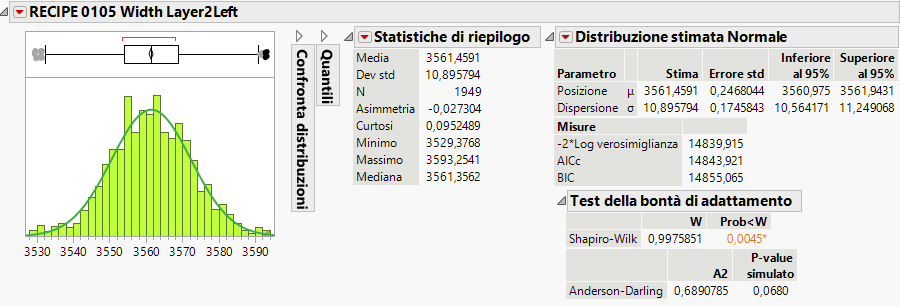
\includegraphics[width=1 \textwidth]{img/Rec105-Normality-Test.png}
  \caption{Goodness of Fit per il codice ricetta 105}
  \label{fig:Rec105-Normality-Test.png}
\end{figure}

Un test di Anderson-Darling pari a 0,689 indica che i dati seguono in modo moderato una distribuzione normale. 
In sintesi, il test di Anderson-Darling e il p value corrispondente è maggiore di 0,005 fanno sì che l'ipotesi nulla (H0) venga accettata e si giunge all'inferenza che per il codice ricetta 105, i dati seguono una distribuzione normale. 


Per la ricetta 103 nella Fig. \ref{fig:Rec103-Normality-Test.png} , la curtosi negativa indica che la distribuzione dei dati ha una forma più piatta rispetto a una distribuzione normale. \\
Il p value minore di 0,005 suggerisce che la distribuzione non è compatibile con una distribuzione normale a un livello di significatività dello 0,05, per cui non è possibile accettare l'ipotesi nulla.


\begin{figure}[h]
  \centering
  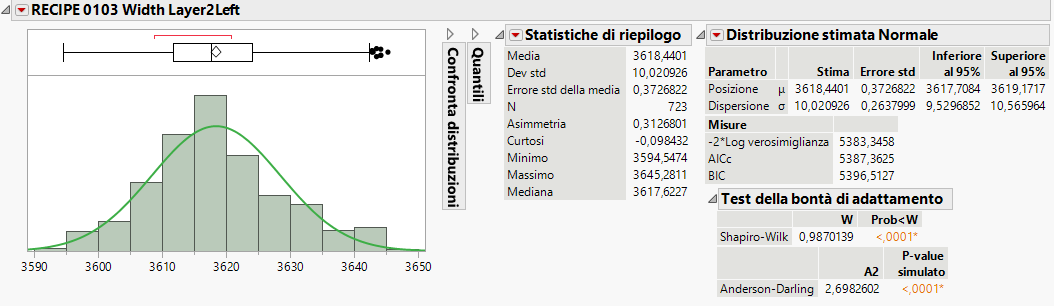
\includegraphics[width=1 \textwidth]{img/Rec103-Normality-Test.png}
  \caption{Goodness of Fit per il codice ricetta 103}
  \label{fig:Rec103-Normality-Test.png}
\end{figure}

Si procederà a fare l'analisi della capacità di processo solo sul codice ricetta 105, ovvero l'unico ad aver soddisfatto l'ipotesi che la distribuzione segua una la forma di una normale.


\label{Costruzione ed analisi degli indici di capacità del processo}
\section{Costruzione ed analisi degli indici di capacità del processo}



Per l'analisi della capacità di processo sono stati considerati il target e i limiti di tolleranza, previsti dal piano di controllo per la variabile della larghezza dell'innerliner.
A tal proposito per il codice ricetta 105 si avrà un valore di target pari a 3550 mm ed una tolleranza di ± 20mm da quest'ultimo.
Nella Fig. \ref{fig:Rec105-Capability.png} é possibile vedere graficamente come si distribuisce il processo attorno ai limiti di specifica.

Qui sottostante l'indice $CP$ calcolato sulla base dell'equazione 2.2:
\begin{equation*} CP = \frac{UTL-LTL}{6\sigma} = \frac{3570-3530}{6 * 10,89579} = 4,665
\label {eqn: CP_105}
\end{equation*}

L'indice $CP$ pari a 4,665 indica che il processo di produzione ha un elevato livello di capacità, il che significa che il processo é in grado di produrre innerliner conformi alle specifiche stabilite nel piano di controllo con una variazione dei dati molto bassa rispetto alle specifiche stesse.
Un valore di $CP$ così elevato indica che il processo è stato attentamente analizzato e che sono state adottate misure per ridurre la variabilità dei dati, questo rappresenta un grande vantaggio in quanto consente di produrre un alto numero di prodotti di alta qualità con un minimo di scarti o difetti. 
Tuttavia, anche con un $CP$ così elevato, è importante mantenere la costante attenzione e la verifica del processo.

Come enunciato in precedenza, l'indice $CP$ è un indicatore efficace della capacità di processo, ma non è sufficiente da solo. 
Il $CP$ controlla solo la dispersione del processo, ma non fornisce informazioni sulla sua centratura. Per questo motivo si farà anche uso dell'indice $CPK$ considerando quindi, anche la posizione centrale delle specifiche rispetto alla media del processo. 

L'indice $CPK$ sarà calcolato sulla base dell'equazione 2.3:
\begin{equation*}CPK = min\left(\frac{UTL-\bar{X}}{3\sigma} ; 
\frac{\bar{X}-LTL}{3\sigma}\right) = min\left(\frac{3570-3561,459}{3*10,89579} ; \frac{3561,459-3530}{3*10,89579}\right) = 1,992
\label {eqn: CPK_105}
\end{equation*}

Un valore di  $CPK$ di 1,992 indica che il processo ha una capacità accettabile di produrre innerliner conformi alle specifiche stabilite dal piano di controllo. 
Tuttavia, la variazione dei dati del processo potrebbe essere leggermente superiore rispetto al valore di target, ciò significa che una percentuale di innerliner prodotti potrebbe non soddisfare appieno le specifiche stabilite.

Anche se il risultato dato dal $CPK$ potrebbe essere migliorabile, un valore di 1,992 è comunque un indicatore che il processo sta funzionando a un buon livello. Ciò significa che il processo è in grado di produrre un elevato numero di innerliner conformi alle specifiche stabilite, ma ci potrebbe essere ancora margine di miglioramento. 
Mantenere una costante attenzione e verifica dei valori rilevati da questo processo, è la chiave per portare a un ulteriore aumento della capacità del processo.

\clearpage
\begin{figure}[h]
  \centering
  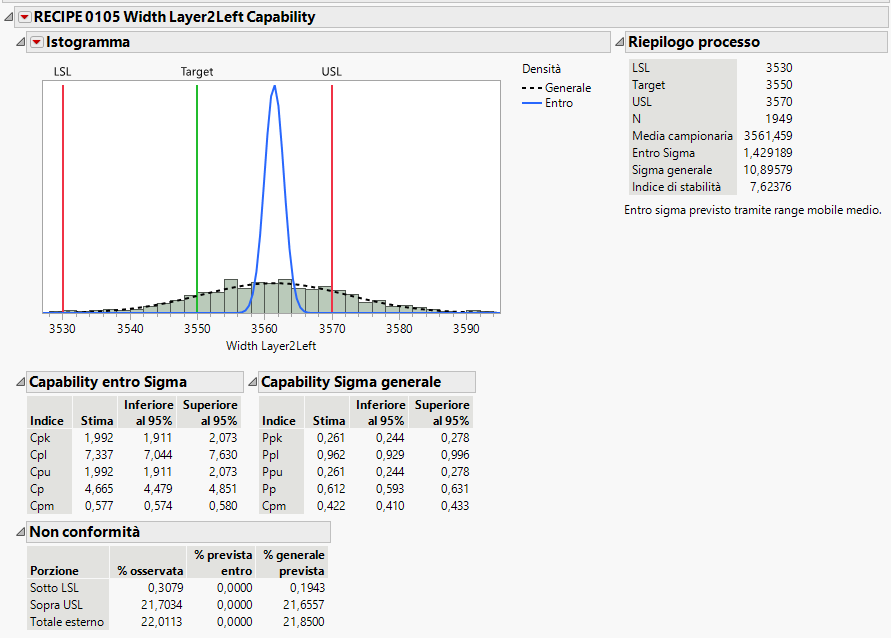
\includegraphics[width=1 \textwidth]{img/Rec105-Capability.png}
  \caption{Capacità del processo del codice ricetta 105 }
  \label{fig:Rec105-Capability.png}
\end{figure}


%%%%%%%%%%%%%%%%%%%%%%%%%%%
Si é scelto di continuare ad analizzare il codice ricetta 103, in una diversa giornata di produzione per osservare in dettaglio se fosse nuovamente presente la variabilità dovuta al fermo macchina.

Per visualizzare meglio l'evoluzione del campione estratto nel tempo di produzione selezionato e attorno ai propri limiti di specifica, si è scelto di sfruttare l'uso della carta di controllo, vedi Cap.\ref{chap:Big Data e l'analisi della capacità di un processo}. 
La carta di controllo del campione estratto nella giornata selezionata è osservabile nella Fig. \ref{fig:Rec-103-ControlChart.png}.
La prima cosa che si nota nel grafico, è la presenza di una delle cause di variabilità: tra le 11:00 e le 12:00 circa c'è un interruzione dei valori rilevati, causata da un fermo macchina, tale situazione rispecchia la medesima analisi del codice ricetta di due giorni precedenti.

È interessante dunque, vedere come si comporta il processo, considerando la presenza una delle cause speciali di variabilità, vedi Fig.\ref{fig:cause.png}.

Il fermo macchina in questione interrompe il flusso del processo, bloccando la produzione per almeno 30 minuti.
Una volta risolto il problema, il funzionamento della macchina viene ripristinato. Tuttavia, potrebbe essere necessario un periodo di tempo per raggiungere nuovamente i livelli di produzione precedenti all'interruzione del processo, questo periodo di tempo viene definito come ``messa a punto''.
Nel momento della messa a punto, i valori rilevati sono ancora in parte influenzati dal ripristino della macchina.
Nella Fig. \ref{fig:Rec-103-ControlChart.png} è possibile vedere tali valori in corrispondenza dei punti di colore rosa.

Per avere una comprensione di come tale causa di variabilità impatta nel processo produttivo, si è proceduto a calcolare gli indici di capacità di processo $CP$ e $CPK$.

Qui sottostante l'indice $CP$ calcolato sulla base dell'equazione 2.2:
\begin{equation*} CP = \frac{UTL-LTL}{6\sigma} = \frac{3580-3620}{6 * 10,021} = 4,441
\label {eqn: CP_103_NEW}
\end{equation*}

L'indice $CP$ ottenuto, è pari a 4,441, un valore poco più basso del risultato ottenuto per il codice ricetta 105, vedi Fig. \ref{fig:Rec105-Capability.png}. 
Ciò indica che il processo di produzione ha un elevato livello di capacità, poco più inferiore rispetto al caso in cui non vi è un fermo macchina, il che potrebbe suggerire che il processo produttivo è ben controllato e la probabilità di produrre prodotti difettosi è molto bassa.

Tuttavia, anche con un $CP$ così elevato, è importante considerare l'indice $CPK$, per osservare come il fermo macchina ha impattato sulla centratura del processo.

L'indice $CPK$ sarà calcolato sulla base dell'equazione 2.3:
\begin{equation*}CPK = min\left(\frac{UTL-\bar{X}}{3\sigma} ; 
\frac{\bar{X}-LTL}{3\sigma}\right) = min\left(\frac{3580-3618,44}{3*10,021} ; \frac{3618,44-3620}{3*10,021}\right) = 0,346
\label {eqn: CPK_105_NEW}
\end{equation*}


Il valore di $CPK$ rilevato, pari a 0,346 suggerisce che il processo produttivo è in parte al di fuori dei limiti di specifica centrali, ovvero la media dei dati del processo non è centrata tra le specifiche di tolleranza. Questo indica che il processo produttivo potrebbe avere una forte tendenza a produrre prodotti difettosi.
Di conseguenza, una parte dei pezzi prodotti del processo cadono oltre i limiti di specifica.
In sintesi, il risultato di $CP$ =  4,441 indica una buona capacità del processo di produrre prodotti all'interno delle specifiche di tolleranza, ma il valore di $CPK$ suggerisce che il processo potrebbe avere problemi di centratura dei dati, che potrebbero portare a produrre prodotti fuori specifica.

Nel Fig. \ref{fig:Rec-103-Capability.png} è possibile visualizzare graficamente come si comporta il processo attorno ai limiti.

In questo caso, la presenza di un fattore di variabilità porta ad un distacco dall'obiettivo di produrre prodotti che riescano a soddisfare appieno le specifiche stabilite.

Lo studio degli indici di capacità di processo ha permesso di identificare il modo in cui la presenza di una causa di variabilità speciale, impatta sulla produzione di innerliner.

\clearpage
\begin{figure}[h]
  \centering
  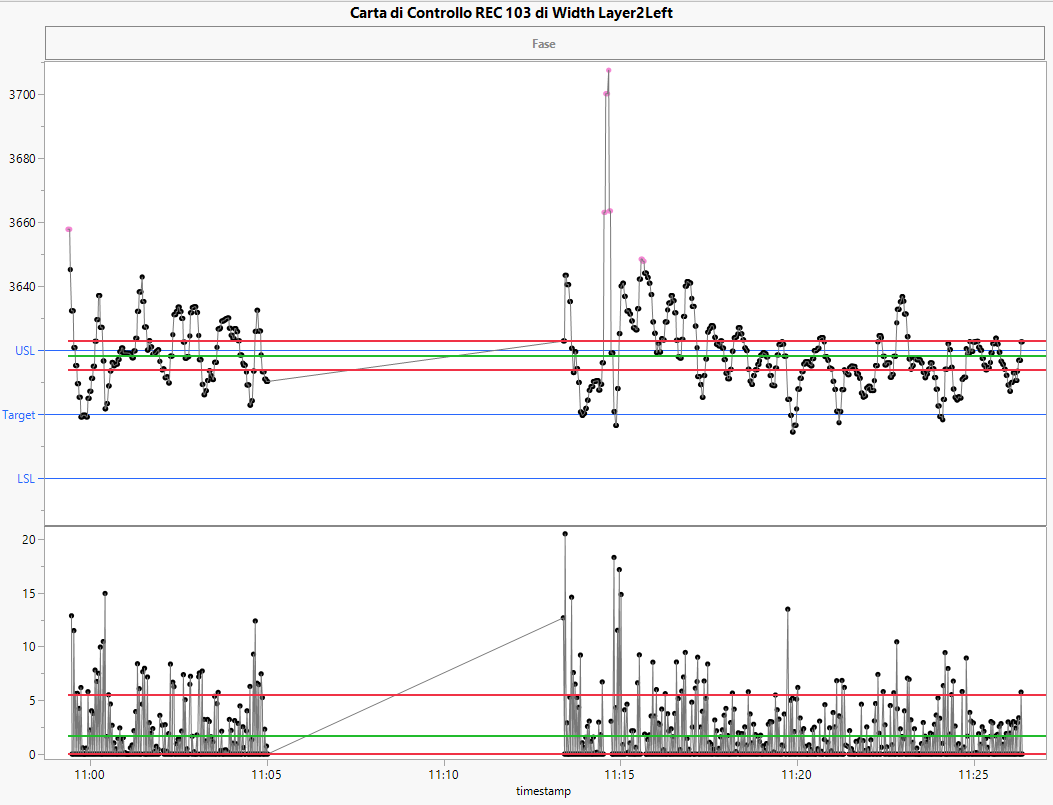
\includegraphics[width=1 \textwidth]{img/Rec-103-ControlChart.png}
  \caption{Carta di controllo del codice ricetta 103 prodotto due giorni successivi}
  \label{fig:Rec-103-ControlChart.png}
\end{figure}


\begin{figure}[h]
  \centering
  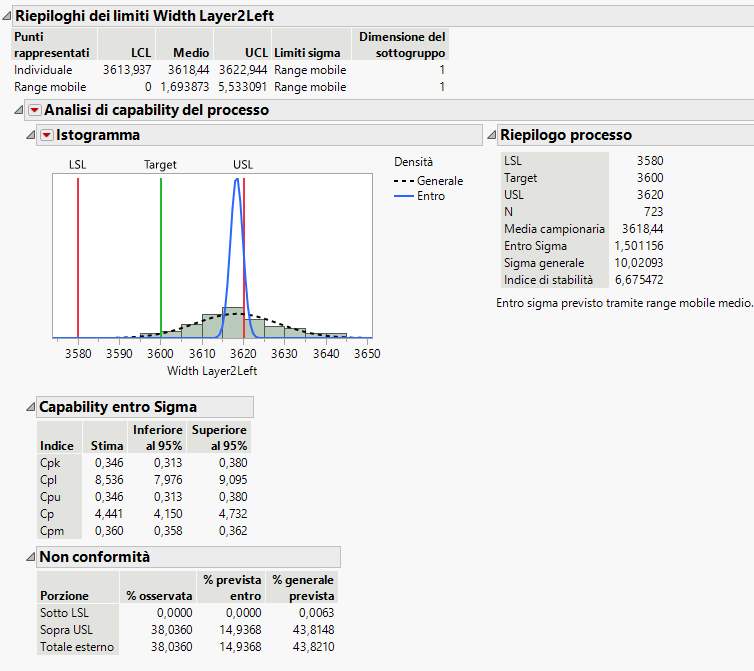
\includegraphics[width=1 \textwidth]{img/Rec-103-Capability.png}
  \caption{Capacità del processo del codice ricetta 103 prodotto due giorni successivi}
  \label{fig:Rec-103-Capability.png}
\end{figure}



%%%%%%%%%%%%%%%%%%%%%%%%%%%%%%%%%%%%%%%%%%%%%%%%%%%%%%%%%%%%%%%%%%%%%%%%%%
%%% CODE FOR PULIZIA DEI DATI PRELIMININARE
% \lstinputlisting[label=lst: strumenti-ottici, firstline=1, lastline=56, caption={Pulizia dei dati}]{code/strumenti-ottici.py}
% %%% CODE


\chapter*{Conclusioni}
\label{chap:Conclusioni}
\markboth{Conlusioni}{Conclusioni}



Il fine del lavoro è lo studio di come sarebbe possibile prevenire gli scarti di produzione, ossia dei prodotti che non rispettano le specifiche richieste. 
Tale obiettivo è stato raggiunto anche attraverso l'applicazione di tecniche statistiche, quali l'analisi della capacità di processo. \\
La metodologia utilizzata è stata quella di monitorare la qualità del prodotto, attraverso una prima validazione ed esplorazione dei dati e delle conseguenti distribuzioni dei parametri di interesse.
Successivamente si é proceduto ad estrarre un campione ed analizzare, tramite l'utilizzo di serie storiche, la distribuzione di questo nell'intervallo di produzione. \\
Grazie allo studio di tale serie storica, dopo aver definito un criterio per la rimozione degli outlier, é stato possibile fare una valutazione di screening del processo per uno specifico codice ricetta, identificando i valori anomali che alteravano il campione.
Al fine di calcolare gli indici di capacità del processo $CP$ e $CPK$, si é reso necessario elaborare un test d'ipotesi per verificare la normalità della distribuzione, essendo quest'ultimo un requisito fondamentale. \\
Successivamente é stato possibile costruire gli indici $CP$ e $CPK$ per ogni specifico codice ricetta, ed identificare attraverso quest'ultimi come si comportava il processo produttivo in presenza e o in assenza di un fermo macchina.

Un'intuizione futura, che potrebbe essere interessante esplorare, è legata ai criteri e alle modalità adottate per l'identificazione dei valori anomali, al fine di ridurre la dispersione dei singoli codici ricetta.

La struttura con la quale vengono raccolti i dati dallo strumento ottico consente di condurre l'analisi della capacità di processo per uno specifico codice di ricetta su ogni ciclo di produzione, ma non in base a lotti composti da diverse bobine prodotte con lo stesso codice di ricetta.

Inoltre, una futura implementazione potrebbe essere quella di valutare la qualità del prodotto associata a ciascuna bobina e di definire una procedura per utilizzare attivamente e correttamente lo strumento di misura online, definendo come e dove misurare le caratteristiche di interesse, sulla base del piano di controllo e della conoscenza del processo.

Ancora, in un'ipotesi di riduzione dei difetti, un uso completo e corretto dello strumento di misura potrebbe migliorare la riduzione degli scarti.
In futuro, il progetto che si intende realizzare e che è attualmente in corso, è quello di automatizzare il processo di raccoglimento dei dati e sincronizzare in tempo reale il calcolo degli indici di processo.
La disponibilità di informazioni in tempo reale, tramite un implementazione di una \textit{Dashboard} sfruttando la tecnologia di Data Visualization, troverebbe il suo utilizzo nel identificare e limitare la variabilità del processo e correlare queste informazioni con gli scarti sul prodotto finito. 

In questo modo, l'analisi di capacità sui semilavorati come l'innerliner, potrebbe essere utile per capire le cause profonde dei diversi tipi di difetti e anche la loro relazione con l'uniformità dello pneumatico.


% \textcolor{red}{L'obiettivo della presente tesi era quello di effettuare XXX. Tale obiettivo è stato raggiunto anche attraverso l'applicazione di tecniche statistiche relative all'analisi di capicità di processo. }
% Grazie all'analisi del caso di studio proposto in tale tesi, dopo aver definito un criterio per la rimozione degli outlier, si 
% \textcolor{red}{FORSE AGGIUNGERE QUALCHE CONSIDERAZIONE}

% \appendix
% INCLUSIONE APPENDICI - - PERSONALIZZARE - TENERE COERENTE CON LISTA IN ALTO
\chapter*{Acronomi utilizzati}

\begin{itemize}
    \item SPC: Controllo Statistico di Processo \textit{(Statistical Process Control)}.
    \item CP: Process Capability
    \item CPK: Process Capability Index
    \item PP: Process Performance
    \item PPK: Process Perfomance Index
    \item UCL: Limite superiore di controllo
    \item CL: Linea Centrale
    \item LCL: Limite inferiore di controllo 
    \item Q1: Primo Quartile
    \item Q3: Terzo Quartile
    \item IQR: Distanza interquartile
    \item UTL: Limite di tolleranza superiore
    \item LTL: Limite di tolleranza inferiore
    \item  $\mathit{\sigma}$: Deviazione standard
    \item $\mathit{\bar{X}}$: Media Campionaria
\end{itemize}




% RINGRAZIAMENTI - PERSONALIZZARE
\ringraziamenti
\rhead{}


....






%%%%%%%%%%%%%%%%%%%%%%%%%%%%%%%%%%%%%%%%%%%%%%%%%%%%%%%%%%%%%%%

%%%%%%%%%%%%%%%%%%%%%% BIBLIOGRAFIA
\phantomsection
\addcontentsline{toc}{chapter}{\refname}
\nocite{*}
\printbibliography

% \cite{paper1} and \cite{paper2} were published later than \citeMath{paper3}. See also \citePhys{paper4}.

% \bibliographystyle{unsrt}
% \bibliography{bibliography}

% \bibliographystyleMath{unsrt}
% \bibliographyMath{sitografia}


\end{document}



